%%%%%%%%%%%%%%%%%%%%%%%%%%%%%%%%%%%%%%%%%%%%%%%%%%%%%%%%%%%%%%%%%%%%%%%%%
%                                                                       %
% ustthesis_test.tex: A template file for usage with ustthesis.cls      %
%                                                                       %
%%%%%%%%%%%%%%%%%%%%%%%%%%%%%%%%%%%%%%%%%%%%%%%%%%%%%%%%%%%%%%%%%%%%%%%%%

\documentclass{ustthesis}

\usepackage{mathpazo,amsmath,amssymb,epsfig,enumerate,bbm,calc,color,ifthen,capt-of} % original was times, but I think it's ugly; we use the same as IEEE CompSoc
\usepackage{algorithm}
%\usepackage[noend]{algorithmic}
\usepackage[center]{subfigure}
\usepackage{color,graphicx}
\newtheorem{proof}{Proof}
\usepackage{hyperref} % for better viewing experience  -- added by alan
\usepackage[margin=25mm,textheight=247mm,textwidth=145mm]{geometry}

% Alan: begin the font trial
% Euler for math | Palatino for rm | Helvetica for ss | Courier for tt
\renewcommand{\rmdefault}{ppl} % rm
%\linespread{1.05}        % Palatino needs more leading
\usepackage[scaled]{helvet} % ss
\usepackage{courier} % tt
%\usepackage{euler} % math
\usepackage{eulervm} % a better implementation of the euler package (not in gwTeX)
\normalfont
\usepackage[T1]{fontenc}
% Alan: end the font trial

\newcommand{\red}[1]{#1}
\newcommand{\tab}[1]{\hspace{3mm}}

\usepackage{epstopdf}
\usepackage{listings}
\usepackage{xcolor}
\usepackage{algpseudocode}
\usepackage{algorithm}
\usepackage{setspace}
\usepackage{tensor}
%%%%%%%%%%%%%%%%%%%%%%%%%%%%%%%%%%%%%%%%%%%%%%%%%%%%%%%%%%%%%%%%%%%%%%%%%
%                                                                       %
% Preambles. DO NOT ERASE THEM. Change to suite your particular purpose.%
%                                                                       %
%%%%%%%%%%%%%%%%%%%%%%%%%%%%%%%%%%%%%%%%%%%%%%%%%%%%%%%%%%%%%%%%%%%%%%%%%

\title{Flocking of Unmanned Aerial Vehicles under Visual Relative Position}    % Title of the thesis.
\author{Xiyuan Liu}                                                         % Author of the thesis.
\degree{\MPhil}                                                             % Degree for which the thesis is.
%% or
%\degree{\PhD}                                                              % Degree for which the thesis is.
\subject{Electronic and Computer Engineering}                              % Subject of the Degree.
\department{Electronic and Computer Engineering}                           % Department to which the thesis is submitted.
\advisor{Prof. Li Qiu}          % Supervisor.
\member{Prof. Shaojie Shen, Thesis Committee Member}     % committee member
\depthead{Prof. Bertram Shi}    % department head.
\defencedate{2019}{08}{25}      % \defencedate{year}{month}{day}.

% NOTE:
%   According to the sample shown in the guidelines, page number is
%   placed below the bottom margin.  However, if the author prefers
%   the page number to be printed above the bottom margin, please
%   activate the following command.

% \PNumberAboveBottomMargin

\begin{document}

%%%%%%%%%%%%%%%%%%%%%%%%%%%%%%%%%%%%%%%%%%%%%%%%%%%%%%%%%%%%%%%%%%%%%%%%%
%                                                                       %
% Now the actual Thesis. The order of output MUST be followed:          %
%                                                                       %
%    1) TITLEPAGE                                                       %
%                                                                       %
% The \maketitle command generates the Title page as well as the        %
% Signature page.                                                       %
%                                                                       %
%%%%%%%%%%%%%%%%%%%%%%%%%%%%%%%%%%%%%%%%%%%%%%%%%%%%%%%%%%%%%%%%%%%%%%%%%

\maketitle

%%%%%%%%%%%%%%%%%%%%%%%%%%%%%%%%%%%%%%%%%%%%%%%%%%%%%%%%%%%%%%%%%%%%%%%%%
%                                                                       %
%     2) DEDICATION (Optional)                                          %
%                                                                       %
% The \dedication and \enddedication commands are optional. If          %
% specified it generates a page for dedication.                         %
%
%%%%%%%%%%%%%%%%%%%%%%%%%%%%%%%%%%%%%%%%%%%%%%%%%%%%%%%%%%%%%%%%%%%%%%%%%

% \dedication
% This is an optional section.
% \enddedication

%%%%%%%%%%%%%%%%%%%%%%%%%%%%%%%%%%%%%%%%%%%%%%%%%%%%%%%%%%%%%%%%%%%%%%%%%
%                                                                       %
%     3) ACKNOWLEDGMENTS                                                %
%                                                                       %
% \acknowledgments and \endacknowledgments defines the                  %
% Acknowledgments of the author of the Thesis.                          %
%                                                                       %
%%%%%%%%%%%%%%%%%%%%%%%%%%%%%%%%%%%%%%%%%%%%%%%%%%%%%%%%%%%%%%%%%%%%%%%%%

\acknowledgments

I would never have completed this work without the help from many people. First of all, I thank my advisor, Professor Li Qiu, for his continuous support and guidance in the process of my MPhil study at HKUST, and for his motivation and patience.

I thank the members of my thesis committee, Professor Bertram Shi and Professor Shaojie Shen for their insightful comments on improving this work.

Last but not least, I thank my parents and my girlfriend Xin Mao, for their mental and spiritual support and encouragement through my graduate study.

\endacknowledgments

%%%%%%%%%%%%%%%%%%%%%%%%%%%%%%%%%%%%%%%%%%%%%%%%%%%%%%%%%%%%%%%%%%%%%%%%%
%                                                                       %
%     4) TABLE OF CONTENTS                                              %
%                                                                       %
%%%%%%%%%%%%%%%%%%%%%%%%%%%%%%%%%%%%%%%%%%%%%%%%%%%%%%%%%%%%%%%%%%%%%%%%%

\tableofcontents

%%%%%%%%%%%%%%%%%%%%%%%%%%%%%%%%%%%%%%%%%%%%%%%%%%%%%%%%%%%%%%%%%%%%%%%%%
%                                                                       %
%     5) LIST OF FIGURES (If Any)                                       %
%                                                                       %
%%%%%%%%%%%%%%%%%%%%%%%%%%%%%%%%%%%%%%%%%%%%%%%%%%%%%%%%%%%%%%%%%%%%%%%%%

\listoffigures

%%%%%%%%%%%%%%%%%%%%%%%%%%%%%%%%%%%%%%%%%%%%%%%%%%%%%%%%%%%%%%%%%%%%%%%%%
%                                                                       %
%     6) LIST OF TABLES (If Any)
%                                                                       %
%%%%%%%%%%%%%%%%%%%%%%%%%%%%%%%%%%%%%%%%%%%%%%%%%%%%%%%%%%%%%%%%%%%%%%%%%

\listoftables

%%%%%%%%%%%%%%%%%%%%%%%%%%%%%%%%%%%%%%%%%%%%%%%%%%%%%%%%%%%%%%%%%%%%%%%%%
%                                                                       %
%     7) ABSTRACT                                                       %
%                                                                       %
% \abstract and \endabstract are used to define a short Abstract for    %
% the Thesis.                                                           %
%                                                                       %
%%%%%%%%%%%%%%%%%%%%%%%%%%%%%%%%%%%%%%%%%%%%%%%%%%%%%%%%%%%%%%%%%%%%%%%%%

\begin{abstract}
This thesis presents the design and implementation of an autonomous tracking algorithm for quadrotors in flocking. Simulation and experiments in both indoor and outdoor GPS-denied environments are presented.
Distributed control and measurement are presented.

\end{abstract}


%%%%%%%%%%%%%%%%%%%%%%%%%%%%%%%%%%%%%%%%%%%%%%%%%%%%%%%%%%%%%%%%%%%%%%%%%
%                                                                       %
%     8) The Actual Contents                                            %
%                                                                       %
% The command \chapters MUST BE USED to ensure that the entire content  %
% of the Thesis is double-spaced (in version 1.0).                      %
%                                                                       %
% However, in version 2.0, \chapters will be automatically added in     %
% the beginning of the first chapter.                                   %
%                                                                       %
%%%%%%%%%%%%%%%%%%%%%%%%%%%%%%%%%%%%%%%%%%%%%%%%%%%%%%%%%%%%%%%%%%%%%%%%%

%%\chapters         % Not necessary with ustthesis.cls (v2.0).

%%%%%%%%%%%%%%%%%%%%%%%%%%%%%%%%%%%%%%%%%%%%%%%%%%%%%%%%%%%%%%%%%%%%%%%%%
%                                                                       %
% Each chapter is defined via the \chapter command. The usual sectional %
% commands of LaTeX are also available.                                 %
%                                                                       %
%%%%%%%%%%%%%%%%%%%%%%%%%%%%%%%%%%%%%%%%%%%%%%%%%%%%%%%%%%%%%%%%%%%%%%%%%

\chapter{Introduction}\label{introduction}

Bird flocking is a natural phenomenon which always appears in group activities like collective hunting, entertainment or migration. Biologists have found that the flocking behavior benefits the entire colony by improving the overall foraging~\cite{Foraging}, predators spotting~\cite{Predator} and propagation~\cite{Propagation} efficiency. Specifically, the allocation of individual tasks, communication and motion control of each agent has determined the main characteristics of the flock system, such as the scalability, robustness and convergence rate. Studies regarding the motion control and the realization of bird flocking with mobile robots, with no doubt, will greatly inspire the human beings.

There are three important criteria to describe a stable flocking system: separation, cohesion and alignment~\cite{Reynolds1987}. Alignment criterion requires each agent to match self's velocity with neighboring flockmates in the mid range, separation criterion requires each agent to repel neighboring flockmates in the short range and cohesion criterion requires each agent to steer neighboring flockmates in the long range. The faster a flock converges from division and the quicker $\psi_{scal}$ (\ref{eq:psi_scal}) gets close to 1, the more robust the system is. $N$ is the number of total agents, $v_i$ is a vector denoting the velocity of $i^{th}$ agent in the flock.

\begin{equation}\label{eq:psi_scal}
\psi_{scal}(t)=\frac{1}{N(N-1)}\sum^N_{i=1}\sum_{j\neq i}\frac{v_i(t)v_j(t)}{|v_i(t)||v_j(t)|}
\end{equation}

To study the individual agents and realize the flocking system, quadrotors or unmanned aerial vehicles (UAVs) are selected owing to their flexibility and mobility in 3D space. Today, the capability of a single UAV has been increasing rapidly, accompanied by the falling prices and improving performance of the communication, sensing and processing hardwares. Meanwhile, the measurement and control of the UAVs in flock realization are expected to be distributed. Realization with distributed measurement requires all the information to be collected by sensors on-board, such as LiDAR, inertial measurement unit (IMU) or camera instead of external positioning systems like GPS~\cite{Vicsek2018}, motion capture system~\cite{Swarm2018,MPC} or real-time kinematic system (RTK). Realization with distributed control requires each UAV to decide its movement with information available at that agent~\cite{MAV2017} instead of executing commands from a central computer~\cite{CAPT,POMDP,Kumar2018} or a leader UAV. The assumption of distributed architecture agrees with the nature that individual agents react to their sensed environment and surrounding neighbors.

There are mainly two methods to achieve UAV flockings at present, virtual structure and behavior-based methods. Virtual structure method treats the entire UAVs as a virtual single rigid body where the relative pose between each UAV and the virtual geometry center is kept~\cite{Virtual2008,Askari2015,Cai2012,RAS,Distributed,LQR2014,VirtualLeader,Bearing2016}, however, internal communication is sometimes inevitable and altering flocking shape is inflexible when facing dynamically changing environment. In behavior-based approach, control functions are separated into variety of function items and the whole function is then formed as the combination of different items~\cite{Zhang2018,Martin2014,Vicsek2018,VLAP,Behavior2004}, however, this method suffers from undesirable local minima and the convergence of the flocking is not promising.

\begin{figure}[htb]
  \centering
  \subfigure[Indoor environment.]{\label{fig:indoor}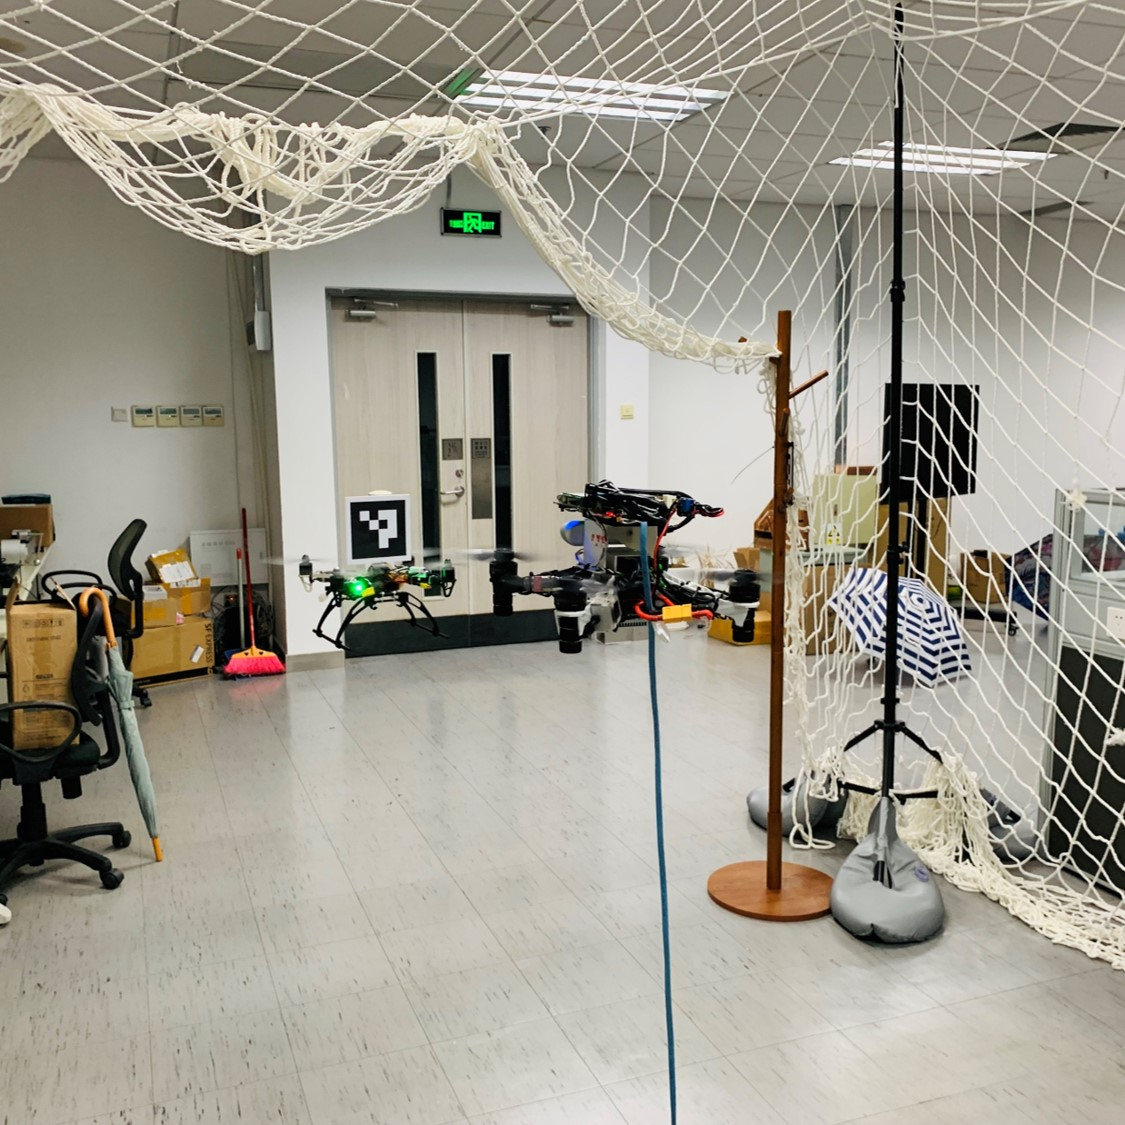
\includegraphics[width=0.49\textwidth]{figure/chapter_1/indoor.jpg}}
  \subfigure[Outdoor environment.]{\label{fig:outdoor}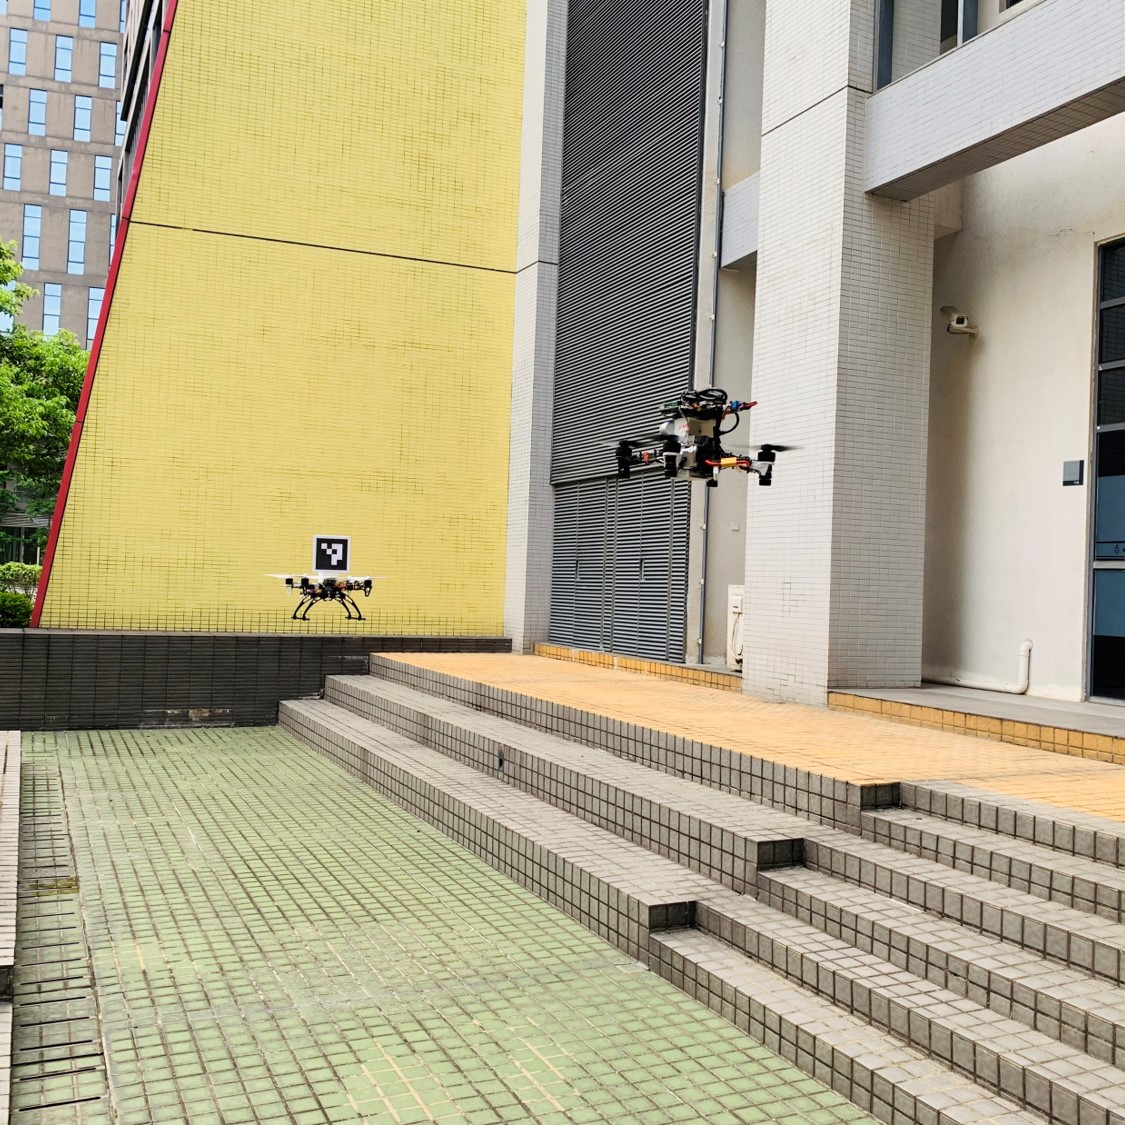
\includegraphics[width=0.49\textwidth]{figure/chapter_1/outdoor.jpg}}
  \caption{Flocking of two UAVs in GPS-denied environments.}\label{fig:indoor_outdoor}
\end{figure}

In this thesis, we present a complete system-level solution to address the aforementioned challenges. The theoretical contribution is the proposal and the proof of a control law satisfying three flocking criteria. The application-level contribution is the design, control and the implementation of the control law using two quadrotors, with the front one being controlled manually and the latter one being fully autonomous as shown in Fig.\ref{fig:indoor_outdoor} and Fig.\ref{fig:twin}. We use the camera as our only on-board sensor for both state estimation and target recognition to maximally imitate natural birds. The flight tests are conducted in both indoor and outdoor environments, and it is successfully demonstrated that our autonomous quadrotor is able to stay flocking with proposed solution.

\begin{figure}[htb]
  \centering
  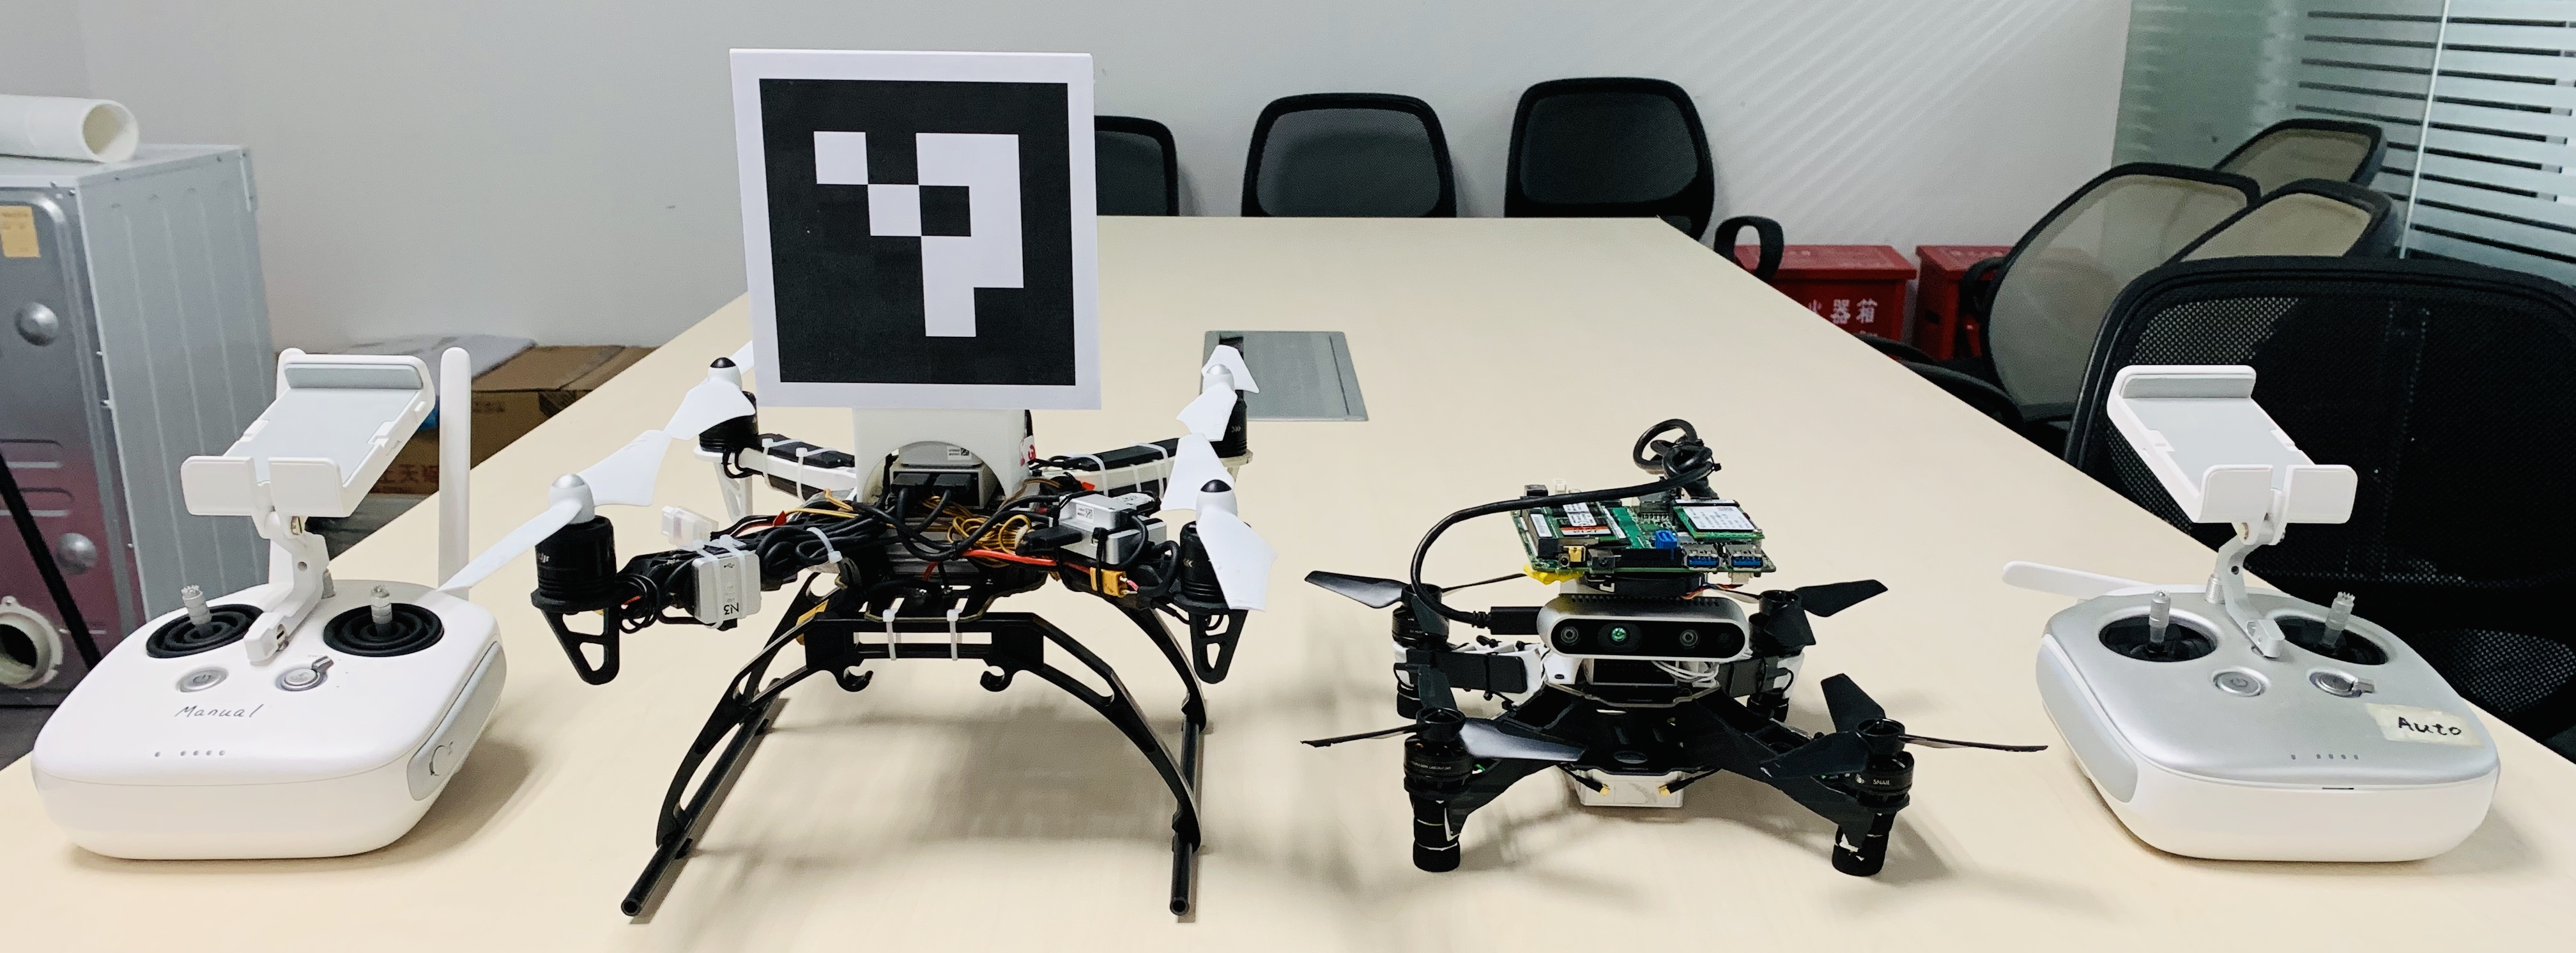
\includegraphics[width=1\textwidth]{figure/chapter_1/all.jpg}
  \caption{Two UAVs where the left one (leader) is manually controlled and the right one (follower) is fully autonomous.}
  \label{fig:twin}
\end{figure}

The outline of the thesis is as follows, Ch.\ref{preliminaries} reviews related theoretical and practical flocking models. Our proposed mathematical model and its proof are shown in Ch.\ref{design}. Ch.\ref{implementation} discusses the architecture and the implementation of our hardware and software platforms. Simulation and real world experiments are shown and in Ch.\ref{experiment}. Ch.\ref{conclusion} concludes this work and points out our possible improvements and future plans.

\newpage

\chapter{Preliminaries and Related Work}\label{preliminaries}

\section{Fixed Topology}\label{flocking}

\subsection{Second-Order System}

Bird flocking or distributed behavior model was first studied in~\cite{Reynolds1987} to animate the aggregate motion in computer simulation. Based on~\cite{Reynolds1987} and observations, a discrete time model (\ref{eq:vicsek}) and the correlation between flock coherence and particle density have been discussed in~\cite{Vicsek1995}. In this model, each particle has a constant velocity, while its direction is determined by ${\langle\theta(t)\rangle}_r$, which is the average direction of the neighboring particles within radius $r$, with $\Delta\theta$ representing the random noise. To clarify the notation, we identify the set of $k$ agents as $V=\{1,...,k\}$ and $x_{ij}=x_i-x_j$, where $x_i$ or $x_i(t)$, $v_i$ or $v_i(t)\in\mathbb{R}^n$ represent the position and velocity of agent $i$ at time $t$ respectively. Unless otherwise noted, we assume the initial positions of the agents are distinct that $x_i(0)\neq x_j(0)$ for $i, j\in V$.

\begin{equation}\label{eq:vicsek}
\begin{aligned}
x_i(t+\Delta t)&=x_i(t)+v_i(t)\Delta t\\
\theta(t+\Delta t)&={\langle\theta(t)\rangle}_r+\Delta\theta
\end{aligned}
\end{equation}

In~\cite{Coordination2013}, the convergence of the model (without noise) in~\cite{Vicsek1995} is proved, however, neither the speeds of birds in nature are constant, nor the headings of birds can be drastically changed that (\ref{eq:vicsek}) cannot be applied for realization. \cite{CuckerSmale2007} has proposed a control law (\ref{eq:motion}, Fig.~\ref{fig:cs_aij}) to resolve the velocity alignment and cohesion problem that the convergence of the flock to a common velocity is guaranteed, however, collision avoidance between agents cannot be assured. Similar protocols including communication delay have been summarized in~\cite{moreau2004stability,ren2005consensus}. The weight $a_{ij}(x):\mathbb{E}^k\to[0,\infty)$ qualifies the influence of agent $j$ acting on agent $i$, which is a function of agent positions. In~\cite{Vicsek1995}, $a_{ij}(x)$ could be equally defined as (\ref{eq:vicsek_aij}).

\begin{equation}\label{eq:motion}
\begin{aligned}
\ddot{x}_i(t)&=\sum^k_{j=1}a_{ij}(x)(v_j-v_i)\\
a_{ij}(x)&=\frac{K}{(\sigma^2+||x_i-x_j||^2)^{\beta}}
\end{aligned}
\end{equation}

\begin{equation}\label{eq:vicsek_aij}
a_{ij}(x)=\left\{\begin{array}{rcl}
1, & & \text{if $||x_i-x_j||\leq$ r}\\
0, & & \text{otherwise}
\end{array} \right.
\end{equation}

Based on~\cite{CuckerSmale2007},~\cite{CuckerDong2010} has further proved the separation of the flocks that the relative distance between each pair of agents will always be greater than a certain lower bound, by appending a collision avoidance term (\ref{eq:dong_aij}). $f(\cdot)$ is a repelling function, $\Lambda(\cdot)$ is a regulating factor and the definition of $a_{ij}(x)$ remains the same as (\ref{eq:motion}). An example of $f(x)=\frac{1}{(x-d_0)^{\theta}}$ is illustrated in Fig.~\ref{fig:dong_f}.

\begin{figure}[htb]
  \centering
  \subfigure[$a_{ij}(x)$ with $\sigma=1$, $K=1$ and $\beta=0.5$ in~\cite{CuckerSmale2007}.]{\label{fig:cs_aij}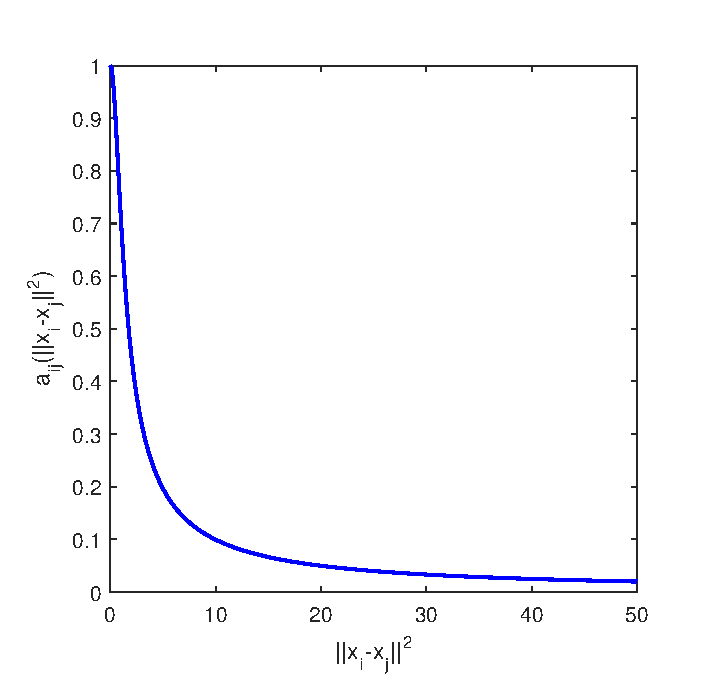
\includegraphics[width=0.32\textwidth]{figure/chapter_2/cs_aij.eps}}
  \subfigure[$f(x)$ with $d_0=1$ and $\theta=2$ in ~\cite{CuckerDong2010}, dashed line represents $x=1$.]{\label{fig:dong_f}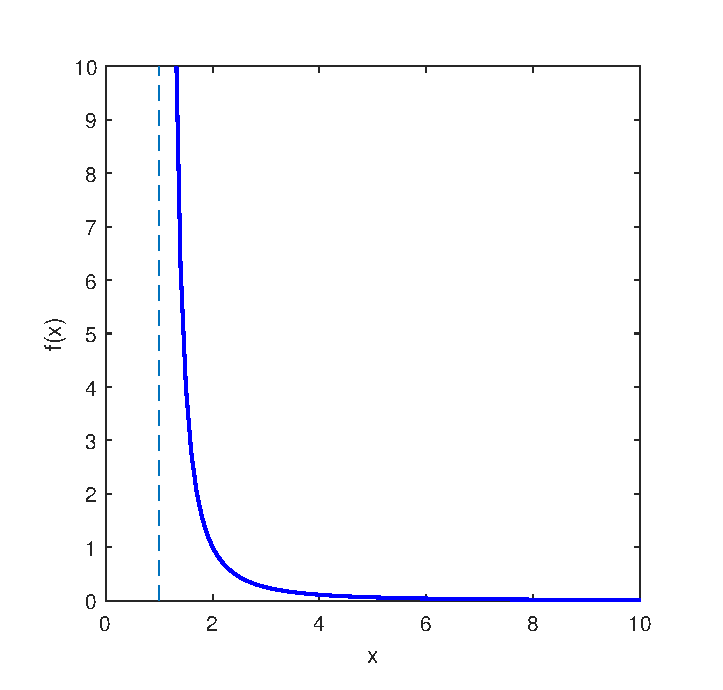
\includegraphics[width=0.32\textwidth]{figure/chapter_2/dong_f.eps}}
  \subfigure[$V_{ij}(x)=\frac{1}{x}+log(x)$, dashed line indicates the global minimum.]{\label{fig:V_ij}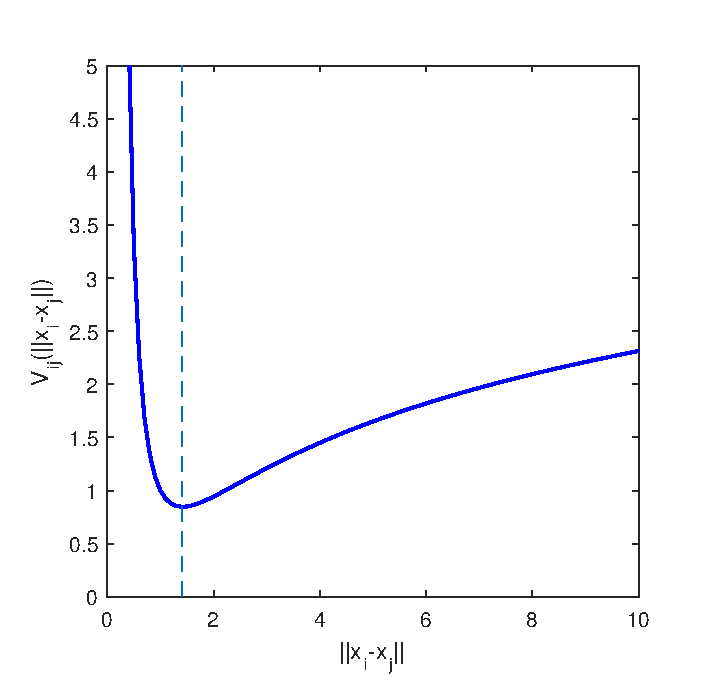
\includegraphics[width=0.32\textwidth]{figure/chapter_2/Vij.eps}}
  \caption{Examples of $a_{ij}(x)$ in~\cite{CuckerSmale2007}, $f(x)$ in~\cite{CuckerDong2010} and $V_{ij}(x)$ in~\cite{FixedTopology}.}\label{fig:example_v}
\end{figure}

\begin{equation}\label{eq:dong_aij}
\begin{aligned}
\ddot{x}_i(t)&=\underbrace{\sum^k_{j=1}a_{ij}(x)(v_j-v_i)}_{\text{velocity consensus term}}+\underbrace{\Lambda(v)\sum_{j\neq i}f(||x_i-x_j||^2)(x_i-x_j)}_{\text{collision avoidance term}}\\
\Lambda(v)&=(\frac{1}{k}\sum_{i>j}||v_i-v_j||^2)^{\frac{1}{2}}
\end{aligned}
\end{equation}

Gradient-based schemes (\ref{eq:fix_topo}) have also been developed in~\cite{FixedTopology,Saber2004,tanner2007flocking,olfati2002distributed} to stabilize inter-agent distances. With the designed artificial potential function $V_{ij}(x)$ (Fig.~\ref{fig:V_ij}) in~\cite{FixedTopology}, the relative distance between agents is expected to locate at the unique minimum. In~\cite{Saber2004}, three flocking rules from~\cite{Reynolds1987}, split, rejoin and squeeze maneuvers have been embodied within their proposed model (\ref{eq:saber}), where $\phi(\cdot)$ is a potential function, $n_{ij}$ is the unit vector along the line connecting $x_i$ and $x_j$ and $a_{ij}$ denotes corresponding adjacency matrix element. When the total number of agents is greater than ten, however, fragmentation may occur that a collective reference pair $(x_r, v_r)$ has to be introduced.

\begin{equation}\label{eq:fix_topo}
\ddot{x}_i(t)=\underbrace{\sum_{j\in V}(v_j-v_i)}_{\text{velocity consensus term}}+\underbrace{(-\sum_{j\in V}\bigtriangledown_{x_i}V_{ij})}_{\text{gradient-based term}}
\end{equation}

\begin{equation}\label{eq:saber}
\ddot{x}_i(t)=\underbrace{\sum_{j\in V}a_{ij}(x)(v_j-v_i)}_{\text{velocity consensus term}}+\underbrace{\sum_{j\in V}\phi(||x_j-x_i||_{\sigma})n_{ij}}_{\text{gradient-based term}}+\underbrace{(-c_1(x_i-x_r)-c_2(v_i-v_r))}_{\text{navigational feedback term}}
\end{equation}

\subsection{First-Order System}

In~\cite{Stability} (\ref{eq:att_rep}),~\cite{Connectedness} (\ref{eq:connect}) and~\cite{Invariant} (\ref{eq:unbound}), first-order control models have been studied that with carefully designed attraction and repulsion functions, Lyapunov function candidates and LaSalle's Invariant Principle, all the flock members are expected to converge to a constant arrangement ($\dot{\mathbf{x}}=0$) within a hyper-ball. Separation is ensured in the first-order system, however, velocity alignment is less satisfied.

\begin{equation}\label{eq:att_rep}
\dot{x}_i=\sum^N_{j=1}(1-e^{-||x_i-x_j||^2})(x_j-x_i)
\end{equation}

\begin{equation}\label{eq:connect}
\dot{x}_i=-\sum_{j\in V}\frac{\partial W_{ij}}{\partial x_i}-\sum_{j\in V}\frac{\partial V_{ij}}{\partial x_i}
\end{equation}

\begin{equation}\label{eq:unbound}
\dot{x}_i=\sum_{j\in V}\frac{2\rho_{ij}}{\gamma_{ij}^2}(D_{ij})_i\mathbf{x}
\end{equation}

\section{Dynamic Topology}

Unlike above mentioned theories assume,~\cite{PNAS} discovered that interaction between agents in flocking does not necessarily depend on the metric distance but rather on the topological distance. An average number of six to seven nearest neighbors are involved in the interaction instead of the whole neighbors within a fixed distance. An example is illustrated in Fig.~\ref{fig:knn}, where the number of nearest neighbors involved $q$ is three. Given conditional initial position, velocity and original $a_{ij}$ in (\ref{eq:vicsek_aij}),~\cite{KNN} has proved that the agents asymptotically agree on a common velocity. Based on~\cite{KNN},~\cite{CuckerDong2016} have further introduced the quotient $\frac{q}{k-1}$ that unconditional flocking occurs when $\frac{q}{k-1}\geq\frac{1}{2}$, where $k$ is the total number of agents.

In~\cite{DynamicTopology}, it is shown that with modified potential function (Fig.~\ref{fig:U_ij}), where the potential is constant when the relative distance between two agents is larger than a certain limit and original model (\ref{eq:fix_topo}), the stability of the flock is guaranteed if no agent is separated initially.

\begin{figure}[H]
  \centering
  \subfigure[A flock of agents with $q=3, k=6$, three closest neighbors of agent 1 and agent 5 are agents 2, 3 and 6 and agents 1, 4 and 6 respectively.]{\label{fig:knn}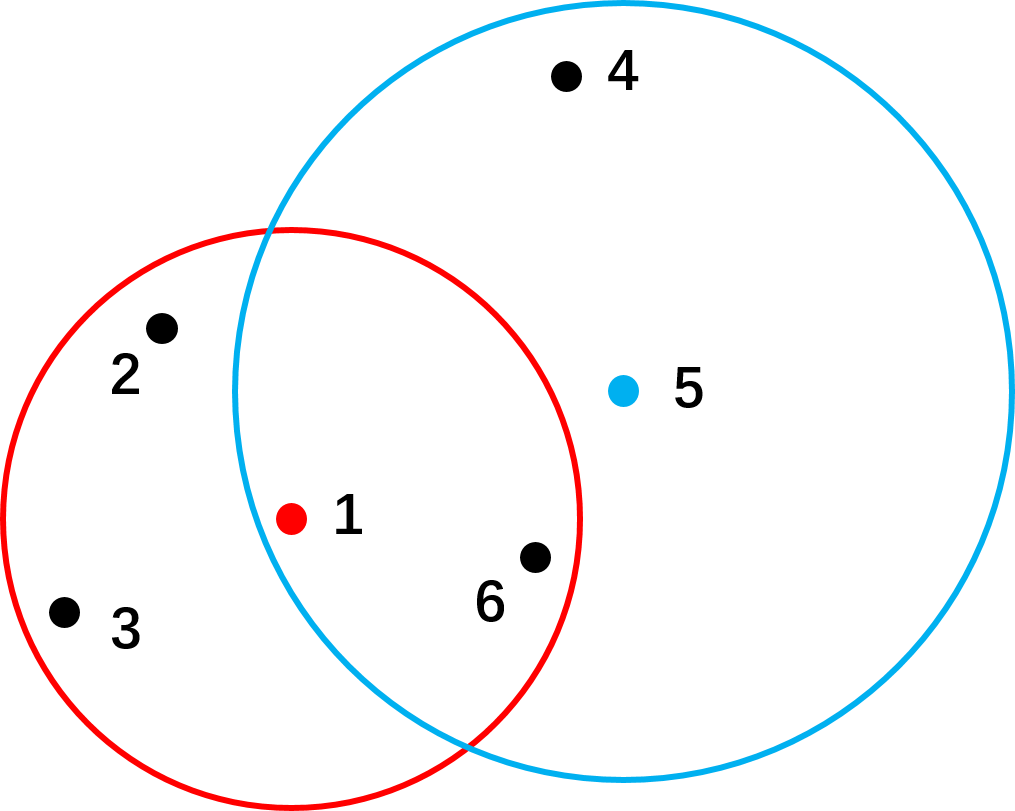
\includegraphics[width=0.4\textwidth]{figure/chapter_2/knn.png}}
  \subfigure[$V_{ij}$ in~\cite{DynamicTopology}. The disconnection of the potential function does not affect the stability.]{\label{fig:U_ij}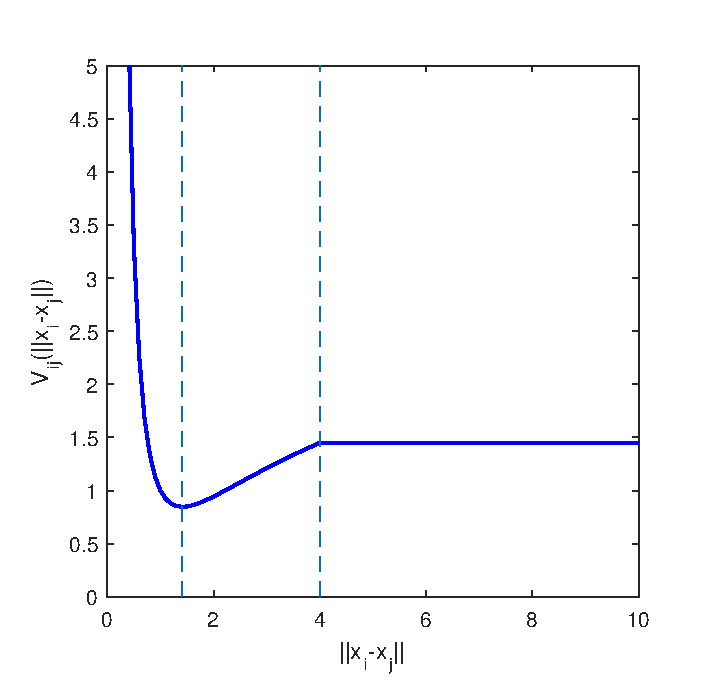
\includegraphics[width=0.4\textwidth]{figure/chapter_2/U.eps}}
  \caption{Examples of dynamic topology and modified potential function.}\label{fig:example_v}
\end{figure}

\newpage

\chapter{Design of Control Model}\label{design}

\section{Proposed Control Law}\label{control_law}

Considering a flock of $k$ agents whose behaviors are described by (\ref{eq:proposed_ui}, \ref{eq:proposed_af}) in continuous time with initial positions satisfying $d_0<||x_i(0)-x_j(0)||^2<d_1$ for all $i\neq j$. At every time step $t$, all agents update their states with the information of the relative positions and velocities between themselves and the neighboring agents. Compared with~\cite{CuckerDong2010}, a cohesion term is appended to the $u_i$ for the purpose of faster convergence and a more compact cohesion. We prove that when $\beta\leq\frac{1}{2}$, the flock will unconditionally converge to a common velocity without collision with other agents. The term $\Lambda(v)$ is designed to adjust the internal repulsion and attraction forces from neighboring agents. Examples of $f_0(x), f_1(x)$ are illustrated in Fig.\ref{fig:f0f1}.

\begin{equation}\label{eq:proposed_ui}
\begin{aligned}
\dot{x_i}(t)&=v_i(t)\\
\dot{v_i}(t)&=u_i(t)\\
u_i(t)&=\underbrace{\sum^k_{j=1}a_{ij}(x)(v_j-v_i)}_{\text{alignment term}}+\\
&\quad\Lambda(v)\underbrace{\sum_{j\neq i}f_0(||x_i-x_j||^2)(x_i-x_j)}_{\text{separation term}}+\\
&\quad\Lambda(v)\underbrace{\sum_{j\neq i}f_1(||x_i-x_j||^2)(x_j-x_i)}_{\text{cohesion term}}
\end{aligned}
\end{equation}

\begin{equation}\label{eq:proposed_af}
\begin{aligned}
a_{ij}(x)&=\frac{K}{(\sigma^2+||x_i-x_j||^2)^{\beta}}\\
\Lambda(v)&=(\frac{1}{k}\sum_{i>j}||v_i-v_j||^2)^{\frac{1}{2}}\\
f_0(x)&=\frac{1}{(x-d_0)^{\theta}}\\
f_1(x)&=\frac{1}{(x-d_1)^{\theta}}
\end{aligned}
\end{equation}

\begin{figure}[htb]
  \centering
  \subfigure[$f_0(x)$ with $d_0=1$]{\label{fig:f0}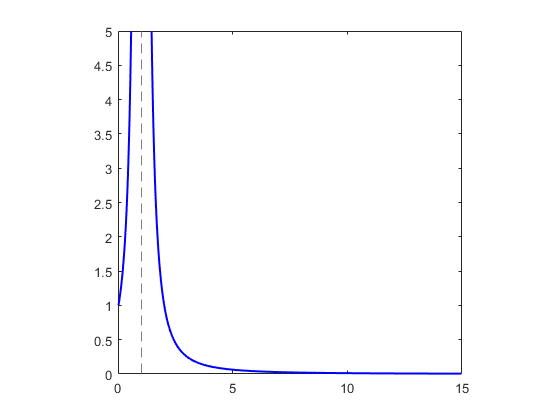
\includegraphics[width=0.48\textwidth]{figure/chapter_3/f0.png}}
  \subfigure[$f_1(x)$ with $d_1=6$]{\label{fig:f1}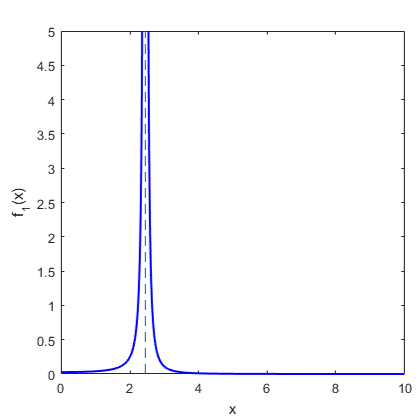
\includegraphics[width=0.48\textwidth]{figure/chapter_3/f1.png}}
  \caption{Examples of $f_0(x), f_1(x)$ in~\ref{eq:proposed_ui}}\label{fig:f0f1}
\end{figure}

\section{Proof of Cohesion and Separation}

Here we omit the detailed proofs of the Lemmas and Propositions originate from~\cite{CuckerDong2010}. Let $F_f$ be the $k$ by $k$ matrix with entries $f_{ij}=f_0(||x_i-x_j||^2)-f_1(||x_i-x_j||^2)$ when $i\neq j$ and $f_{ii}=0$. Let $D_f$ be the Laplacian of $F_f$ which is a diagonal matrix whose entries are $d_{ii}=\sum_{j=1}^k f_{ij}$. We have $L_f=D_f-F_f$. Similarly we have $L_x=D_x-A_x$ where $a_{ij}$ is defined in \ref{eq:proposed_af}. Then (\ref{eq:proposed_ui}) could be equally defined as

\begin{equation}\label{eq:continuous}
\begin{aligned}
\mathbf{\dot{x}}&=\mathbf{v}\\
\mathbf{\dot{v}}&=-L_x\mathbf{v}+\Lambda(v)L_f\mathbf{x}\\
\end{aligned}
\end{equation}

\noindent
where $\mathbf{x}=(x_1, x_2, \dots, x_k)^T$ and $\mathbf{v}=(v_1, v_2, \dots, v_k)^T$. Noticed that matrix $L_x$ acts on $\mathbb{E}^K$ by mapping $(v_1, v_2, \dots, v_k)^T$ to $((L_x)_{i1}v_1+\dots+(L_x)_{ik}v_k)_{i\leq k}$.

Let $\{\bigtriangleup={(u, u, \dots, u)|u\in\mathbb{E}}\}$ be the diagonal of $\mathbb{E}^K$, and $\bigtriangleup^{\perp}$ be the orthogonal complement of $\bigtriangleup$ in $\mathbb{E}^K$. Then we could decompose every element $e\in\mathbb{E}^K=e_{\bigtriangleup}+e^{\perp}$ with $e_{\bigtriangleup}\in\bigtriangleup$ and $e^{\perp}\in\bigtriangleup^{\perp}$. We then decompose $\mathbf{v}=\mathbf{v_{\bigtriangleup}+v^{\perp}}$ where $\mathbf{v_{\bigtriangleup}}=(\bar{v}, \bar{v}, \dots, \bar{v})^T$ and $\mathbf{v^{\perp}}=(v_1-\bar{v}, \dots, v_k-\bar{v})$. $\bar{v}$ is the average velocity of all $k$ agents. We show that $<\mathbf{v_{\bigtriangleup}}, \mathbf{v^{\perp}}>=\sum_{i=1}^k<\bar{v},v_i-\bar{v}>=<\bar{v},\sum_{i=1}^k(v_i-\bar{v})>=0$.

$\mathbf{Lemma 1}$: For any solution $(\mathbf{x}(t), \mathbf{v}(t))$ of (\ref{eq:continuous}), we have $\frac{d}{dt}\mathbf{v}_{\bigtriangleup}=0$.

From Lemma 1, we know that $\mathbf{v_{\bigtriangleup}}$ is constant with $t$ and $a_{ij}(x)=a_{ij}(x^{\perp})$. Thus in the following paragraphs, we use $x$ and $v$ to denote $x^{\perp}$ and $v^{\perp}$ respectively. The system in (\ref{eq:continuous}) then becomes the following

\begin{equation}\label{eq:continuous_projection}
\begin{aligned}
\mathbf{\dot{x}}&=\mathbf{v}\\
\mathbf{\dot{v}}&=-L_x\mathbf{v}+||v||L_f\mathbf{x}\\
\end{aligned}
\end{equation}

Define the function $E: \mathbb{E}^k\times\mathbb{E}^k\to(0,\infty)$ by (\ref{eq:Exv}), where $\delta$ is an infinitesimal positive number.

\begin{equation}\label{eq:Exv}
\begin{aligned}
E(x, v)&=||v||+\frac{1}{2}\sum_{i>j}\int_{||x_i-x_j||^2}^{d_1-\delta}f_0(r)dr-\frac{1}{2}\sum_{i>j}\int_{||x_i-x_j||^2}^{d_1-\delta}f_1(r)dr\\
&=||v||+\frac{1}{2}\sum_{i>j}\int_{||x_i-x_j||^2}^{d_1-\delta}(f_0(r)-f_1(r))dr
\end{aligned}
\end{equation}

$\mathbf{Proposition 1}$: For all $t>0$, $-Hk||v||+<L_fx, v>\leq\frac{d}{dt}||v||\leq-\frac{Hk||v||}{(1+2||x||^2)^{\beta}}+<L_fx, v>$.

$\mathbf{Lemma 2}$: Let $A$ be a $k\times k$ positive, symmetric matrix and $L$ be its Laplacian. Then for all $u, w\in\mathbb{E}^K$ (and in particular, for all $u, w\in\bigtriangleup^{\perp}$), $<w, Lu>=\sum_{i>j}<w_i-w_j, u_i-u_j>a_{ij}$.

\noindent
Using Proposition 1, Lemma 2 and the fundamental theorem of calculus we see the derivative of $E$ along the solution satisfies

\begin{equation}\label{eq:dExv}
\begin{aligned}
\frac{d}{dt}E(x(t), v(t))&=\frac{d}{dt}||v(t)||+\frac{1}{2}\sum_{i>j}\frac{d}{dt}\int_{||x_i(t)-x_j(t)||^2}^{d_1-\delta}(f_0(r)-f_1(r))dr\\
&=\frac{d}{dt}||v(t)||-\frac{1}{2}\sum_{i>j}\frac{d}{dt}<x_i(t)-x_j(t),x_i(t)-x_j(t)>(f_0(||x_i(t)-x_j(t)||^2)\\
&\quad\ -f_1(||x_i(t)-x_j(t)||^2))\\
&\leq-\frac{Hk}{(1+2||x||^2)^{\beta}}||v||+<L_fx, v>-\sum_{i>j}<x_i-x_j, v_i-v_j>(f_0(||x_i-x_j||^2)\\
&\quad-f_1(||x_i-x_j||^2))\\
&=-\frac{Hk}{(1+2||x||^2)^{\beta}}||v||
\end{aligned}
\end{equation}

\noindent
Hence $E(\mathbf{x}(t), \mathbf{v}(t))$ is a decreasing function of t along the solution $(\mathbf{x}(t), \mathbf{v}(t))$. Write

\begin{equation}\label{eq:E0}
E(0)=||v(0)||+\frac{1}{2}\sum_{i>j}\int_{||x_i(0)-x_j(0)||^2}^{d_1-\delta}(f_0(r)-f_1(r))dr
\end{equation}

\noindent
Then for all $t\geq0$, $E(\mathbf{x}(t), \mathbf{v}(t))\leq E(0)$. This implies

\begin{equation}
\frac{1}{2}\sum_{i>j}\int_{||x_i-x_j||^2}^{d_1-\delta}(f_0(r)-f_1(r))dr<E(0)
\end{equation}

\noindent
From the definition of $f_0$ and $f_1$ and the initial conditions that we have ensured $d_0<||x_i(t)-x_j(t)||^2<d_1$ for all $i\neq j$ and $t\geq0$, otherwise the integral in (\ref{eq:Exv}) will go to infinity.

\section{Proof of Velocity Convergence}

Here, we show the proof for the case $\beta\leq\frac{1}{2}$, as the proof for $\beta>\frac{1}{2}$ is similar. From (\ref{eq:dExv}) we could obtain (\ref{eq:Et_E0}, \ref{eq:intE0})

\begin{equation}\label{eq:Et_E0}
E(t)-E(0)\leq-\int_0^t\frac{Hk}{(1+2||x(s)||^2)^{\beta}}||v(s)||ds
\end{equation}

\begin{equation}\label{eq:intE0}
\int_0^t\frac{Hk}{(1+2||x(s)||^2)^{\beta}}||v(s)||ds\leq E(0)
\end{equation}

$\mathbf{Proposition 2}$: For all $t>0$, $\frac{d}{dt}||x(t)||\leq||v(t)||$.

By Proposition 2, we have

\begin{equation}\label{eq:proposition2}
\frac{d}{dt}||x(t)||\leq||v(t)||
\end{equation}

\begin{equation}
\int_{||x(0)||}^{||x(t)||}\frac{Hk}{(1+2y^2)^{\beta}}dy\leq E(0)
\end{equation}

\begin{equation}
\begin{aligned}
E(0)&\geq\int_{||x(0)||}^{||x(t)||}\frac{Hk}{(1+2y^2)^{\beta}}dy\geq\int_{||x(0)||}^{||x(t)||}\frac{Hky}{(1+2y^2)^{\beta+\frac{1}{2}}}dy\\
&=\left\{\begin{array}{rcl}\frac{Hk}{2-4\beta}(1+2y^2)^{\frac{1}{2}-\beta}|^{||x(t)||}_{||x(0)||}, & & \text{if $\beta\neq\frac{1}{2}$}\\\frac{Hk}{4}ln(1+2y^2)|^{||x(t)||}_{||x(0)||}, & & \text{if $\beta=\frac{1}{2}$}\end{array} \right.
\end{aligned}
\end{equation}

\noindent
Assume $||x(t)||$ is unbounded for $t>0$, then as $t\to\infty$, $E(0)\to\infty$ which contradicts with our initial condition. Thus $||x(t)||$ is bounded which leads to

\begin{equation}\label{eq:boundv}
\int_0^{\infty}||v(t)||dt<\infty
\end{equation}

\noindent
We show that $||v(t)||$ is a continuous function of $t$ that

\begin{equation}
\begin{aligned}
|\frac{d}{dt}||v(t)|||&\leq Hk||v(t)||+|<L_fx(t), v(t)>|\\
&=Hk||v(t)||+|\sum_{i>j}f(||x_i(t)-x_j(t)||^2)<v_i-v_j, x_i-x_j>|\\
&\leq Hk||v(t)||+\sum_{i>j}f(||x_i(t)-x_j(t)||^2)||v_i-v_j|| ||x_i-x_j||\leq\infty
\end{aligned}
\end{equation}

\noindent
Then we show that when $t\to\infty$, $||v(t)||\to0$. Assumes there exist some $\delta>0$ that when $t\to\infty$, $||v(t)||\to\delta$, then

\begin{equation}
\int_0^{\infty}||v(t)||dt\geq\infty
\end{equation}

\noindent
which contradicts (\ref{eq:boundv}).

\newpage

\chapter{Implementation on Quadrotors}\label{implementation}

In this chapter, the system architecture is presented, including the software and hardware configurations, specifications of the UAV platform and details of sensors.

\section{Quadrotor Model}

\subsection{Coordinate Frame}

\begin{figure}[htb]
  \centering
  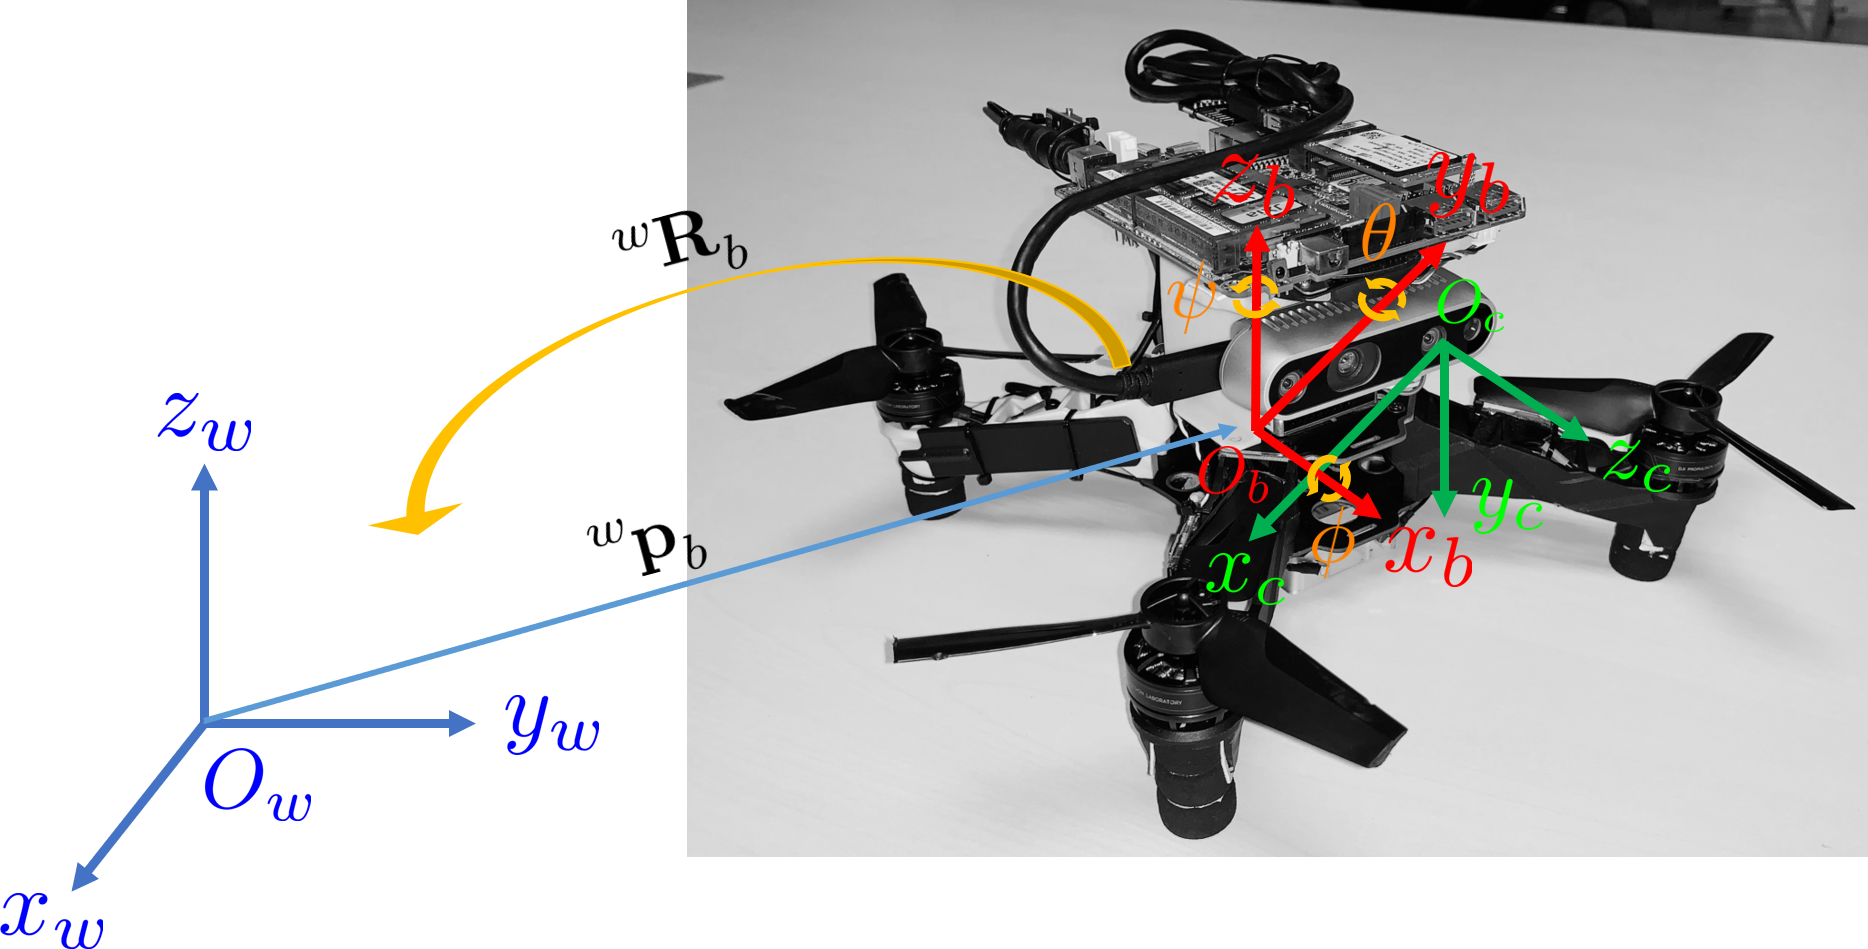
\includegraphics[width=1.0\textwidth]{figure/chapter_4/coordinate.png}
  \caption{Coordinate frames of world, quadrotor body and on-board camera}
  \label{fig:coordinate}
\end{figure}

Three coordinate frames are introduced including world, quadrotor body and its on-board camera as illustrated in Figure~\ref{fig:coordinate}. In Chapter~\ref{implementation}, target quadrotor is captured in camera frame whose position is denoted by $\mathbf{p_c}\in\mathbb{R}^3$. For the simplicity and unity of the calculations, $\mathbf{p_c}$ is transformed back to world frame $\mathbf{p_w}\in\mathbb{R}^3$ by $\tensor*[^w]{\mathfrak{g}}{_c}\in\mathbb{R}^{4\times4}$:

\begin{equation}\label{eq:transform}
\begin{aligned}
\begin{bmatrix}\mathbf{p^T_w}&1\end{bmatrix}^T&=\tensor*[^w]{\mathfrak{g}}{_c}\begin{bmatrix}\mathbf{p^T_c}&1\end{bmatrix}^T\\
\tensor*[^w]{\mathfrak{g}}{_c}&=\tensor*[^w]{\mathfrak{g}}{_b}\tensor*[^b]{\mathfrak{g}}{_c}=\begin{bmatrix}\mathbf{\tensor*[^w]{R}{_b}}&\mathbf{\tensor*[^w]{p}{_b}}\\\mathbf{0^{1\times3}}&1\end{bmatrix}
\begin{bmatrix}\mathbf{\tensor*[^b]{R}{_c}}&\mathbf{\tensor*[^b]{p}{_c}}\\\mathbf{0^{1\times3}}&1\end{bmatrix}\\
\tensor*[^b]{\mathbf{R}}{_c}&=\mathbf{R_z}(\psi)\mathbf{R_y}(\theta)\mathbf{R_x}(\phi)
\end{aligned}
\end{equation}

where $\mathbf{p_c}$ is first rotated w.r.t $z_c$ by yaw angle $\psi$, then $z_y$ by pitch angle $\theta$, last $z_x$ by roll angle $\phi$ and shifted by $\tensor*[^b]{\mathbf{p}}{_c}$ to $\mathbf{p_b}$ in body frame. Iteratively, $\mathbf{p_c}$ is transformed back to $\mathbf{p_W}$ in world frame (\ref{eq:transform}). It is worthwhile to point out that both $\tensor*[^b]{\mathfrak{g}}{_c}$ and $\tensor*[^w]{\mathfrak{g}}{_b}$ are estimated online by ~\cite{VINS} in Chapter~\ref{hardware}. The $\mathbf{R_z}(\psi)$, $\mathbf{R_y}(\theta)$ and $\mathbf{R_x}(\phi)\in\mathfrak{SE(3)}$ are rotation matrixes.

\begin{equation}\label{eq:rotation}
\begin{aligned}
R_z(\psi)&=\begin{bmatrix}cos\psi&-sin\psi&0\\sin\psi&cos\psi&0\\0&0&1\end{bmatrix}\\
R_y(\theta)&=\begin{bmatrix}cos\theta&0&sin]\theta\\0&1&0\\-sin\theta&0&cos\theta\end{bmatrix}\\
R_x(\phi)&=\begin{bmatrix}1&0&0\\0&cos\phi&-sin]\phi\\0&sin\phi&cos\phi\end{bmatrix}
\end{aligned}
\end{equation}

\subsection{Quadrotor Dynamics and Kinematics}

The center of mass of quadrotor body in world frame is denoted by $\mathbf{r}\in\mathbb{R}^3$, then from Newton's law we have:
\begin{equation}\label{eq:newton}
m\mathbf{\ddot{r}}=\begin{bmatrix}0\\0\\-mg\end{bmatrix}+\tensor*[^w]{\mathbf{R}}{_b}\begin{bmatrix}0\\0\\\sum F_i\end{bmatrix}
\end{equation}
where $\mathit{m}\in\mathbb{R}$ is the total weight of the quadrotor and $\mathit{F_i}\in\mathbb{R}$ is the lifting force provided by each motor. The components of the angular velocities of quadrotor in its body frame are denoted by $\mathit{p}$, $\mathit{q}$ and $\mathit{r}\in\mathbb{R}$ and are related with $\theta$, $\phi$ and $\psi\in\mathbb{R}$ by:
\begin{equation}\label{eq:pqr}
\begin{bmatrix}p\\q\\r\end{bmatrix}=\begin{bmatrix}cos\theta&0&-cos\phi sin\theta\\0&1&sin\phi\\sin\theta&0&cos\phi cos\theta\end{bmatrix}\begin{bmatrix}\dot{\phi}\\\dot{\theta}\\\dot{\psi}\end{bmatrix}
\end{equation}

In addition to force, each motor has also produced moment, $\mathit{M_i}\in\mathbb{R}$, perpendicular to $x_b-x_y$ plane. We denote the length from each motor to the center of mass by $\mathit{L}\in\mathbb{R}$ and the moment of inertia matrix along $x_b-y_b-z_b$ axes by $\mathbf{I}\in\mathbb{R}^{3\times3}$. We then have the following Euler equations:\textcolor{red}{TODO: Modify Euler equations}
\begin{equation}\label{eq:euler}
\mathbf{I}\begin{bmatrix}\dot{p}\\\dot{q}\\\dot{r}\end{bmatrix}=\begin{bmatrix}L(F_2-F_4)\\L(F_3-F_1)\\M_1-M_2+M_3-M_4\end{bmatrix}-\begin{bmatrix}p\\q\\r\end{bmatrix}\times
\mathbf{I}\begin{bmatrix}p\\q\\r\end{bmatrix}
\end{equation}

\begin{figure}[htb]
  \centering
  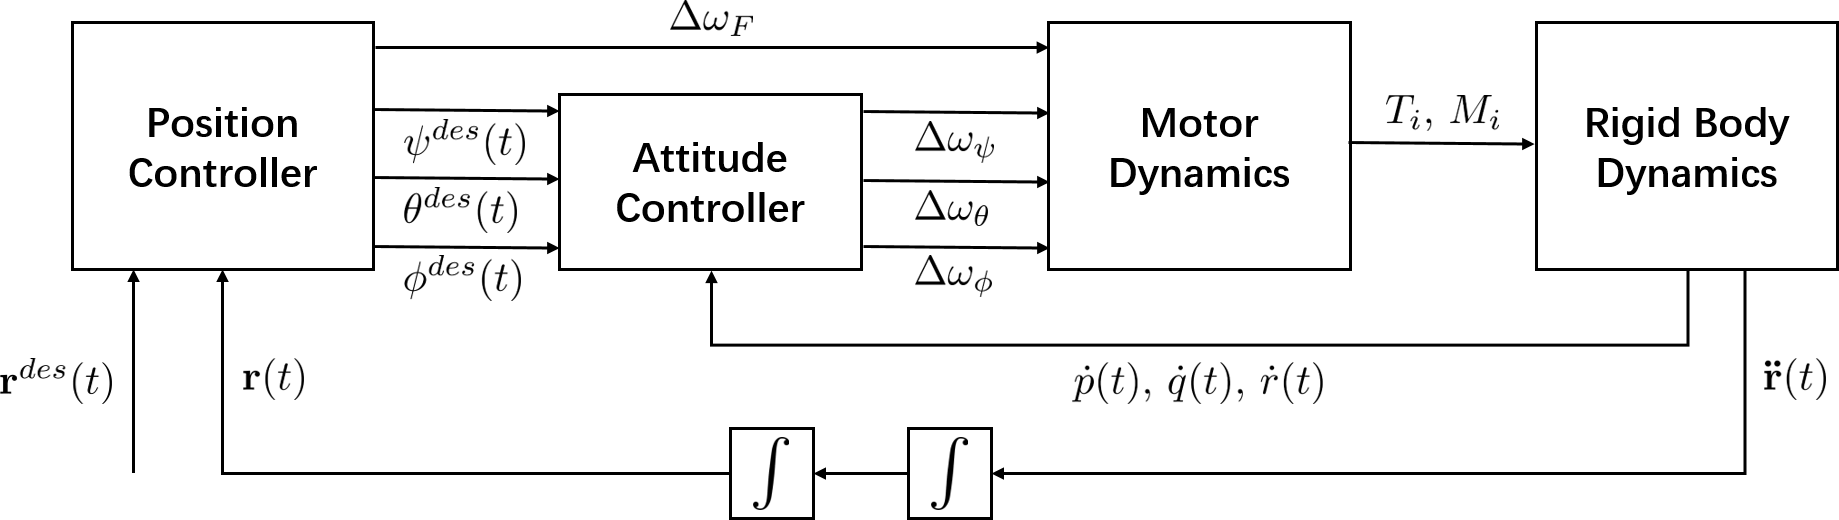
\includegraphics[width=1.0\textwidth]{figure/chapter_2/nest.png}
  \caption{Nested control loops for position and attitude control,~\cite{GRASP}}
  \label{fig:nest}
\end{figure}

As shown in Figure~\ref{fig:nest}, the control loops are divided into inner attitude control and outer position control. With the help of DJI Onboard SDK and owing to the differential flatness property, the state and input could be represented as algebraic functions of four carefully selected flat outputs $[\mathbf{r}^T, \psi]$ and their derivatives~\cite{Snap}. This facilitates the generation of trajectories since any smooth trajectory (with reasonably bounded derivatives) in the space of flat outputs can be followed by the quadrotor. Thus the main work of quadrotor motion planning goes to the design of the required trajectory.

\section{Hardware architecture}\label{hardware}

\begin{figure}[ht]
  \centering
  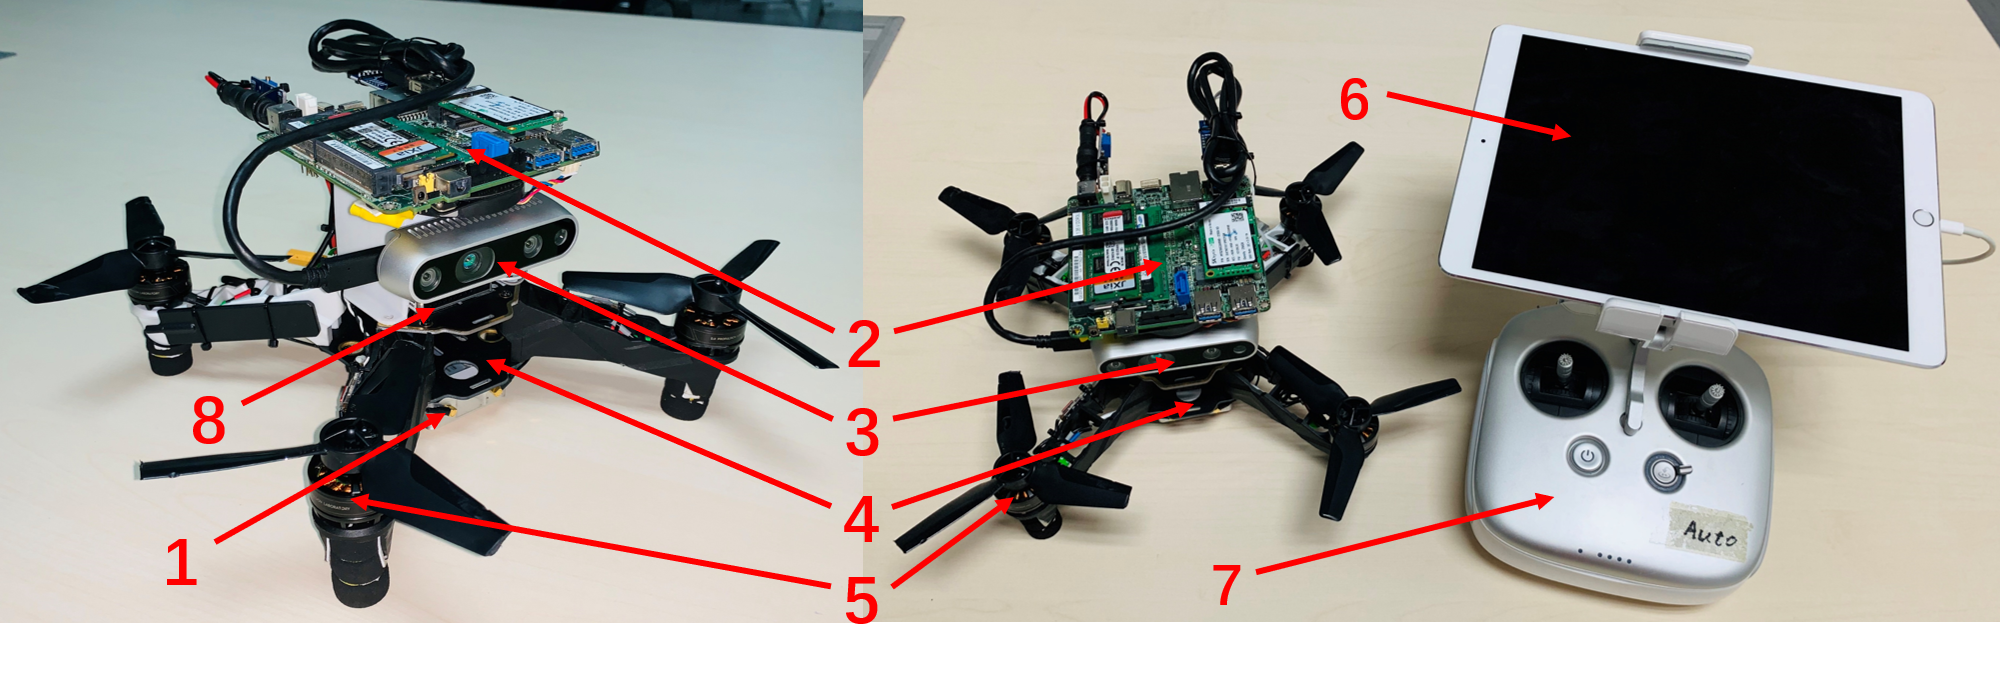
\includegraphics[width=1.0\textwidth]{figure/chapter_4/chaser_intro.png}
  \caption{Chaser quadrotor and remote controller panel: (1) Lightbridge 2 receiver; (2) Intel NUC mini computer; (3) Intel Realsense camera; (4) 4S LiPo Batter Case; (5) DJI snail motor; (6) iPad Live streaming panel; (7) DJI Lightbridge 2 remote controller; (8) DJI N3 flight controller.}
  \label{fig:quadrotor_controller}
\end{figure}

The hardware of UAV platform includes one chaser quadrotor, one target quadrotor and their remote controllers (RCs) as shown in Figure~\ref{fig:quadrotor_controller},~\ref{fig:target_uav}. The quadrotor is first controlled by the RC to take off, then the control authority is switched to on-board mini computer by RC to achieve autonomous driving. The RC has higher control authority than on-board computer that human operator could prevent quadrotor from fatal errors by switching control priority back to RC.

\begin{figure}[htb]
  \centering
  \subfigure[Back]{\label{fig:back}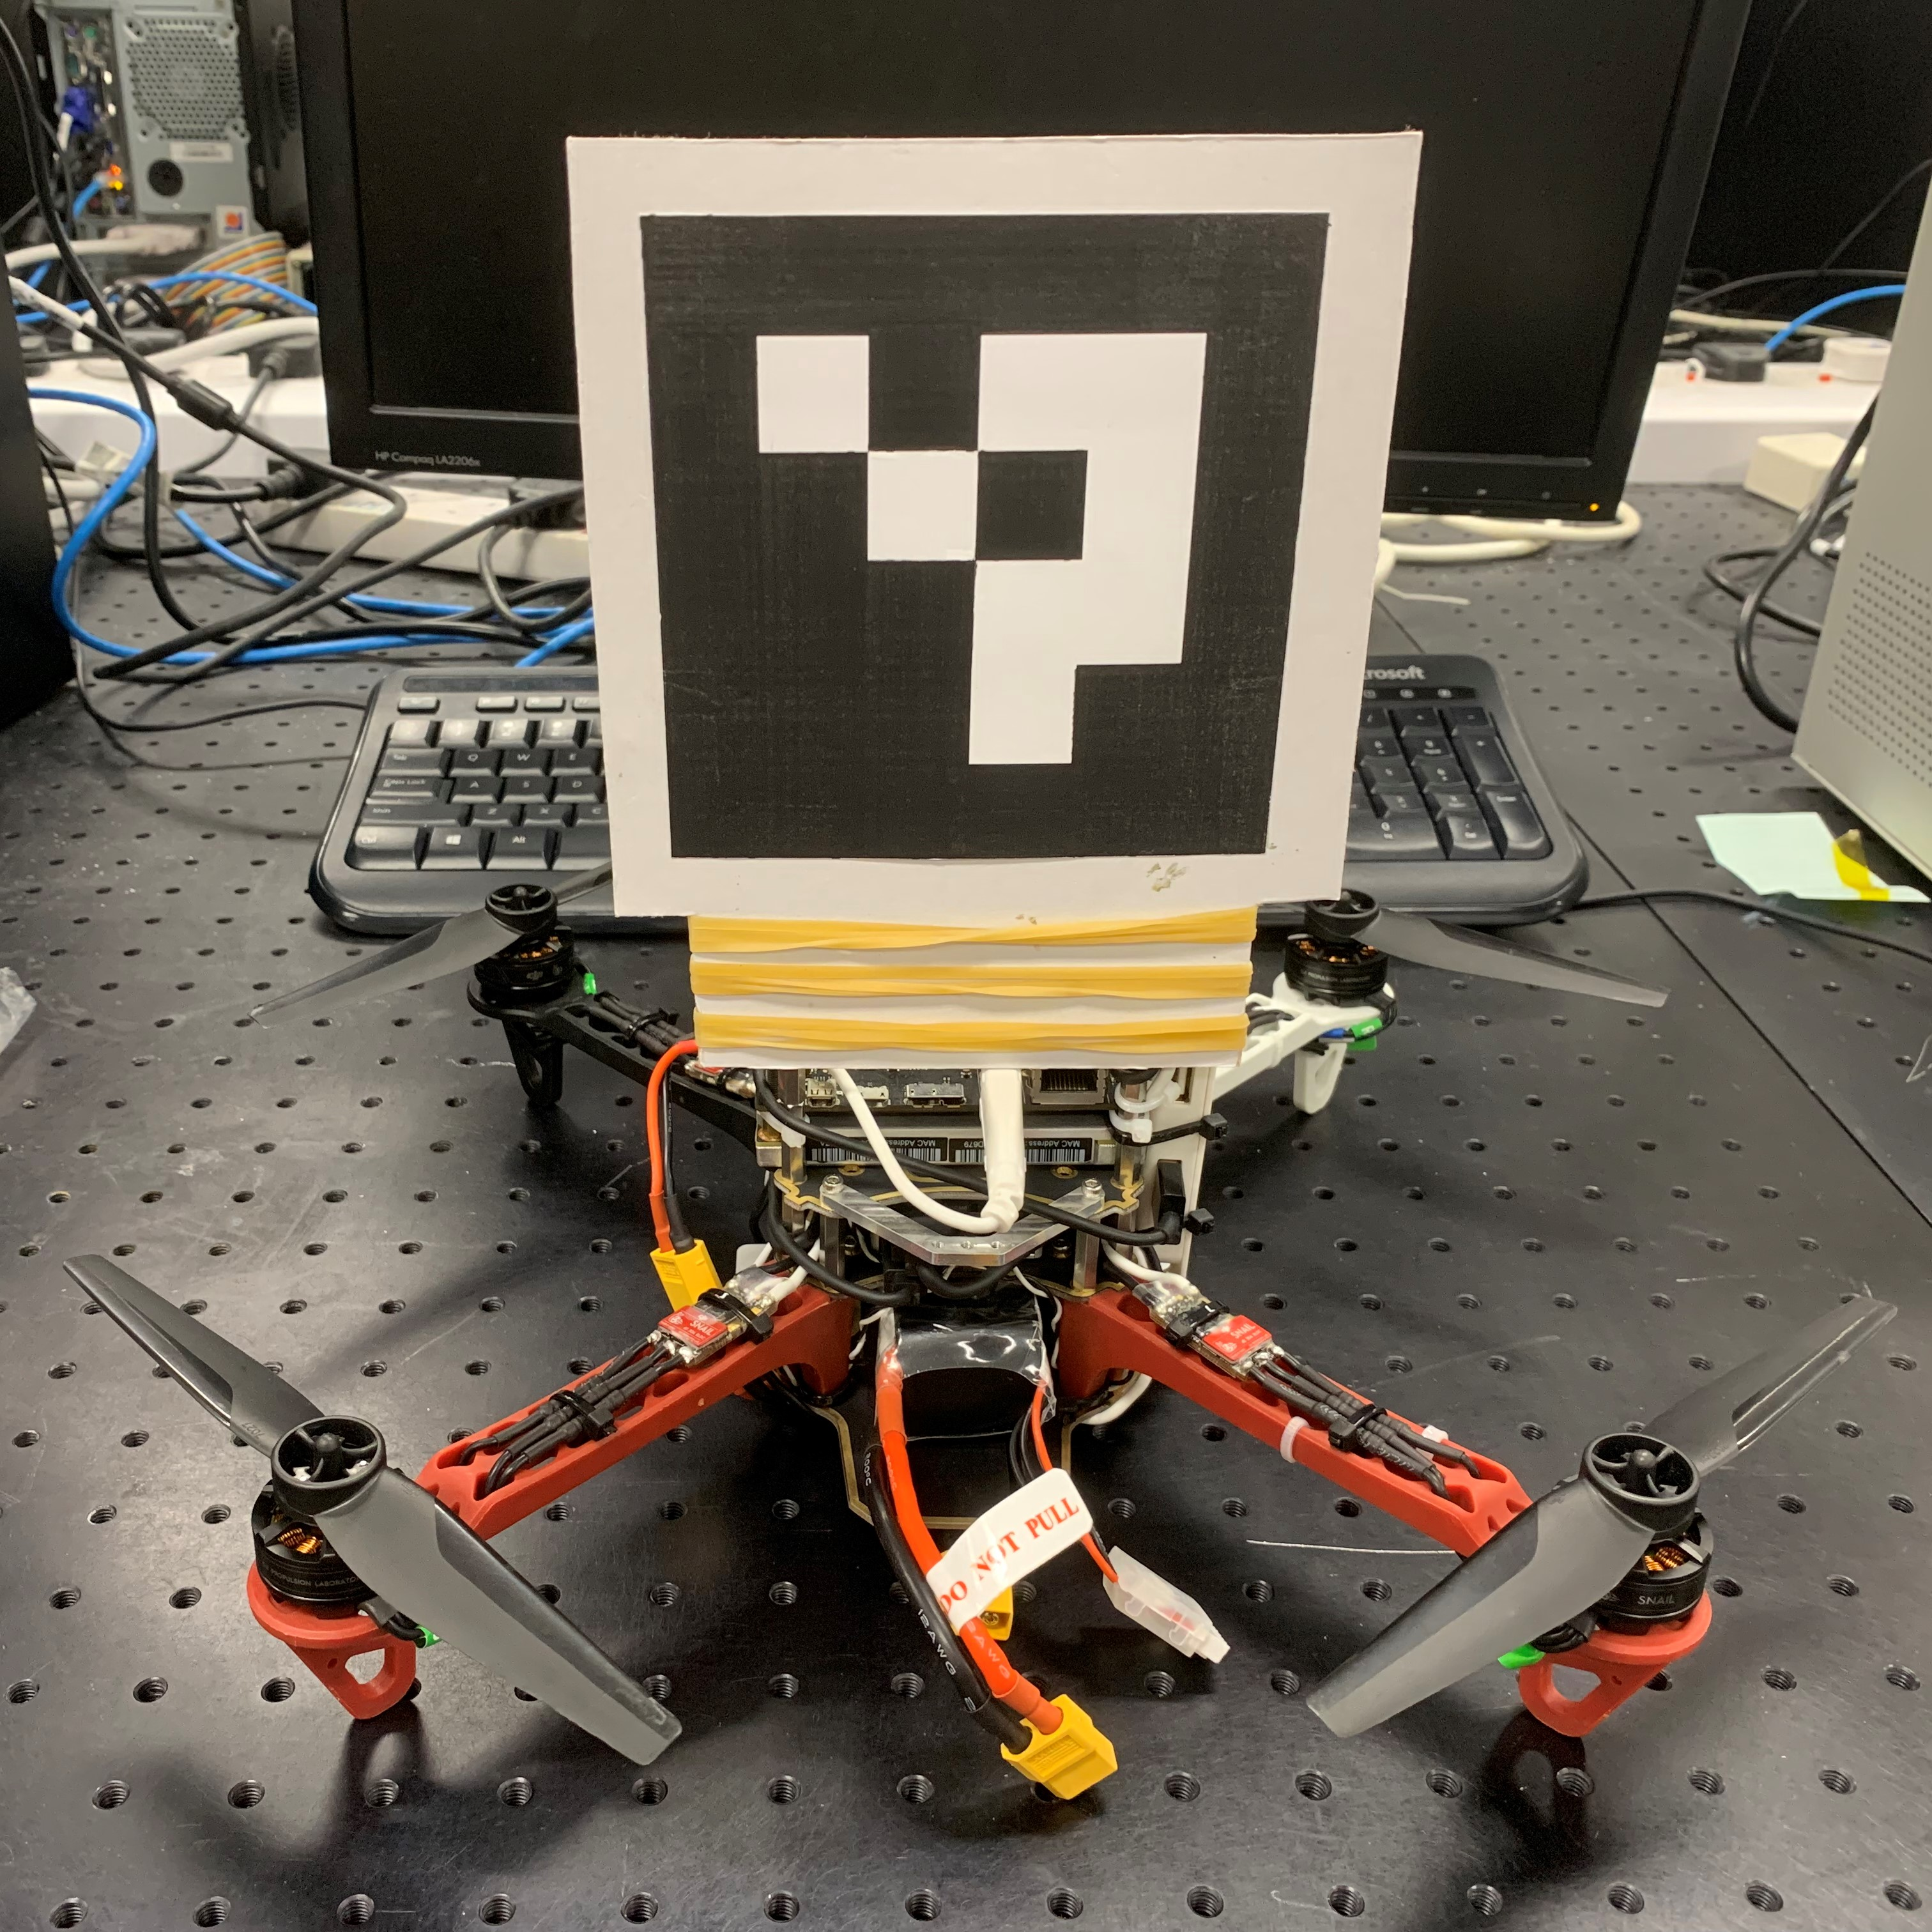
\includegraphics[width=0.49\textwidth]{figure/chapter_4/leader_back.jpg}}
  \subfigure[Front]{\label{fig:front}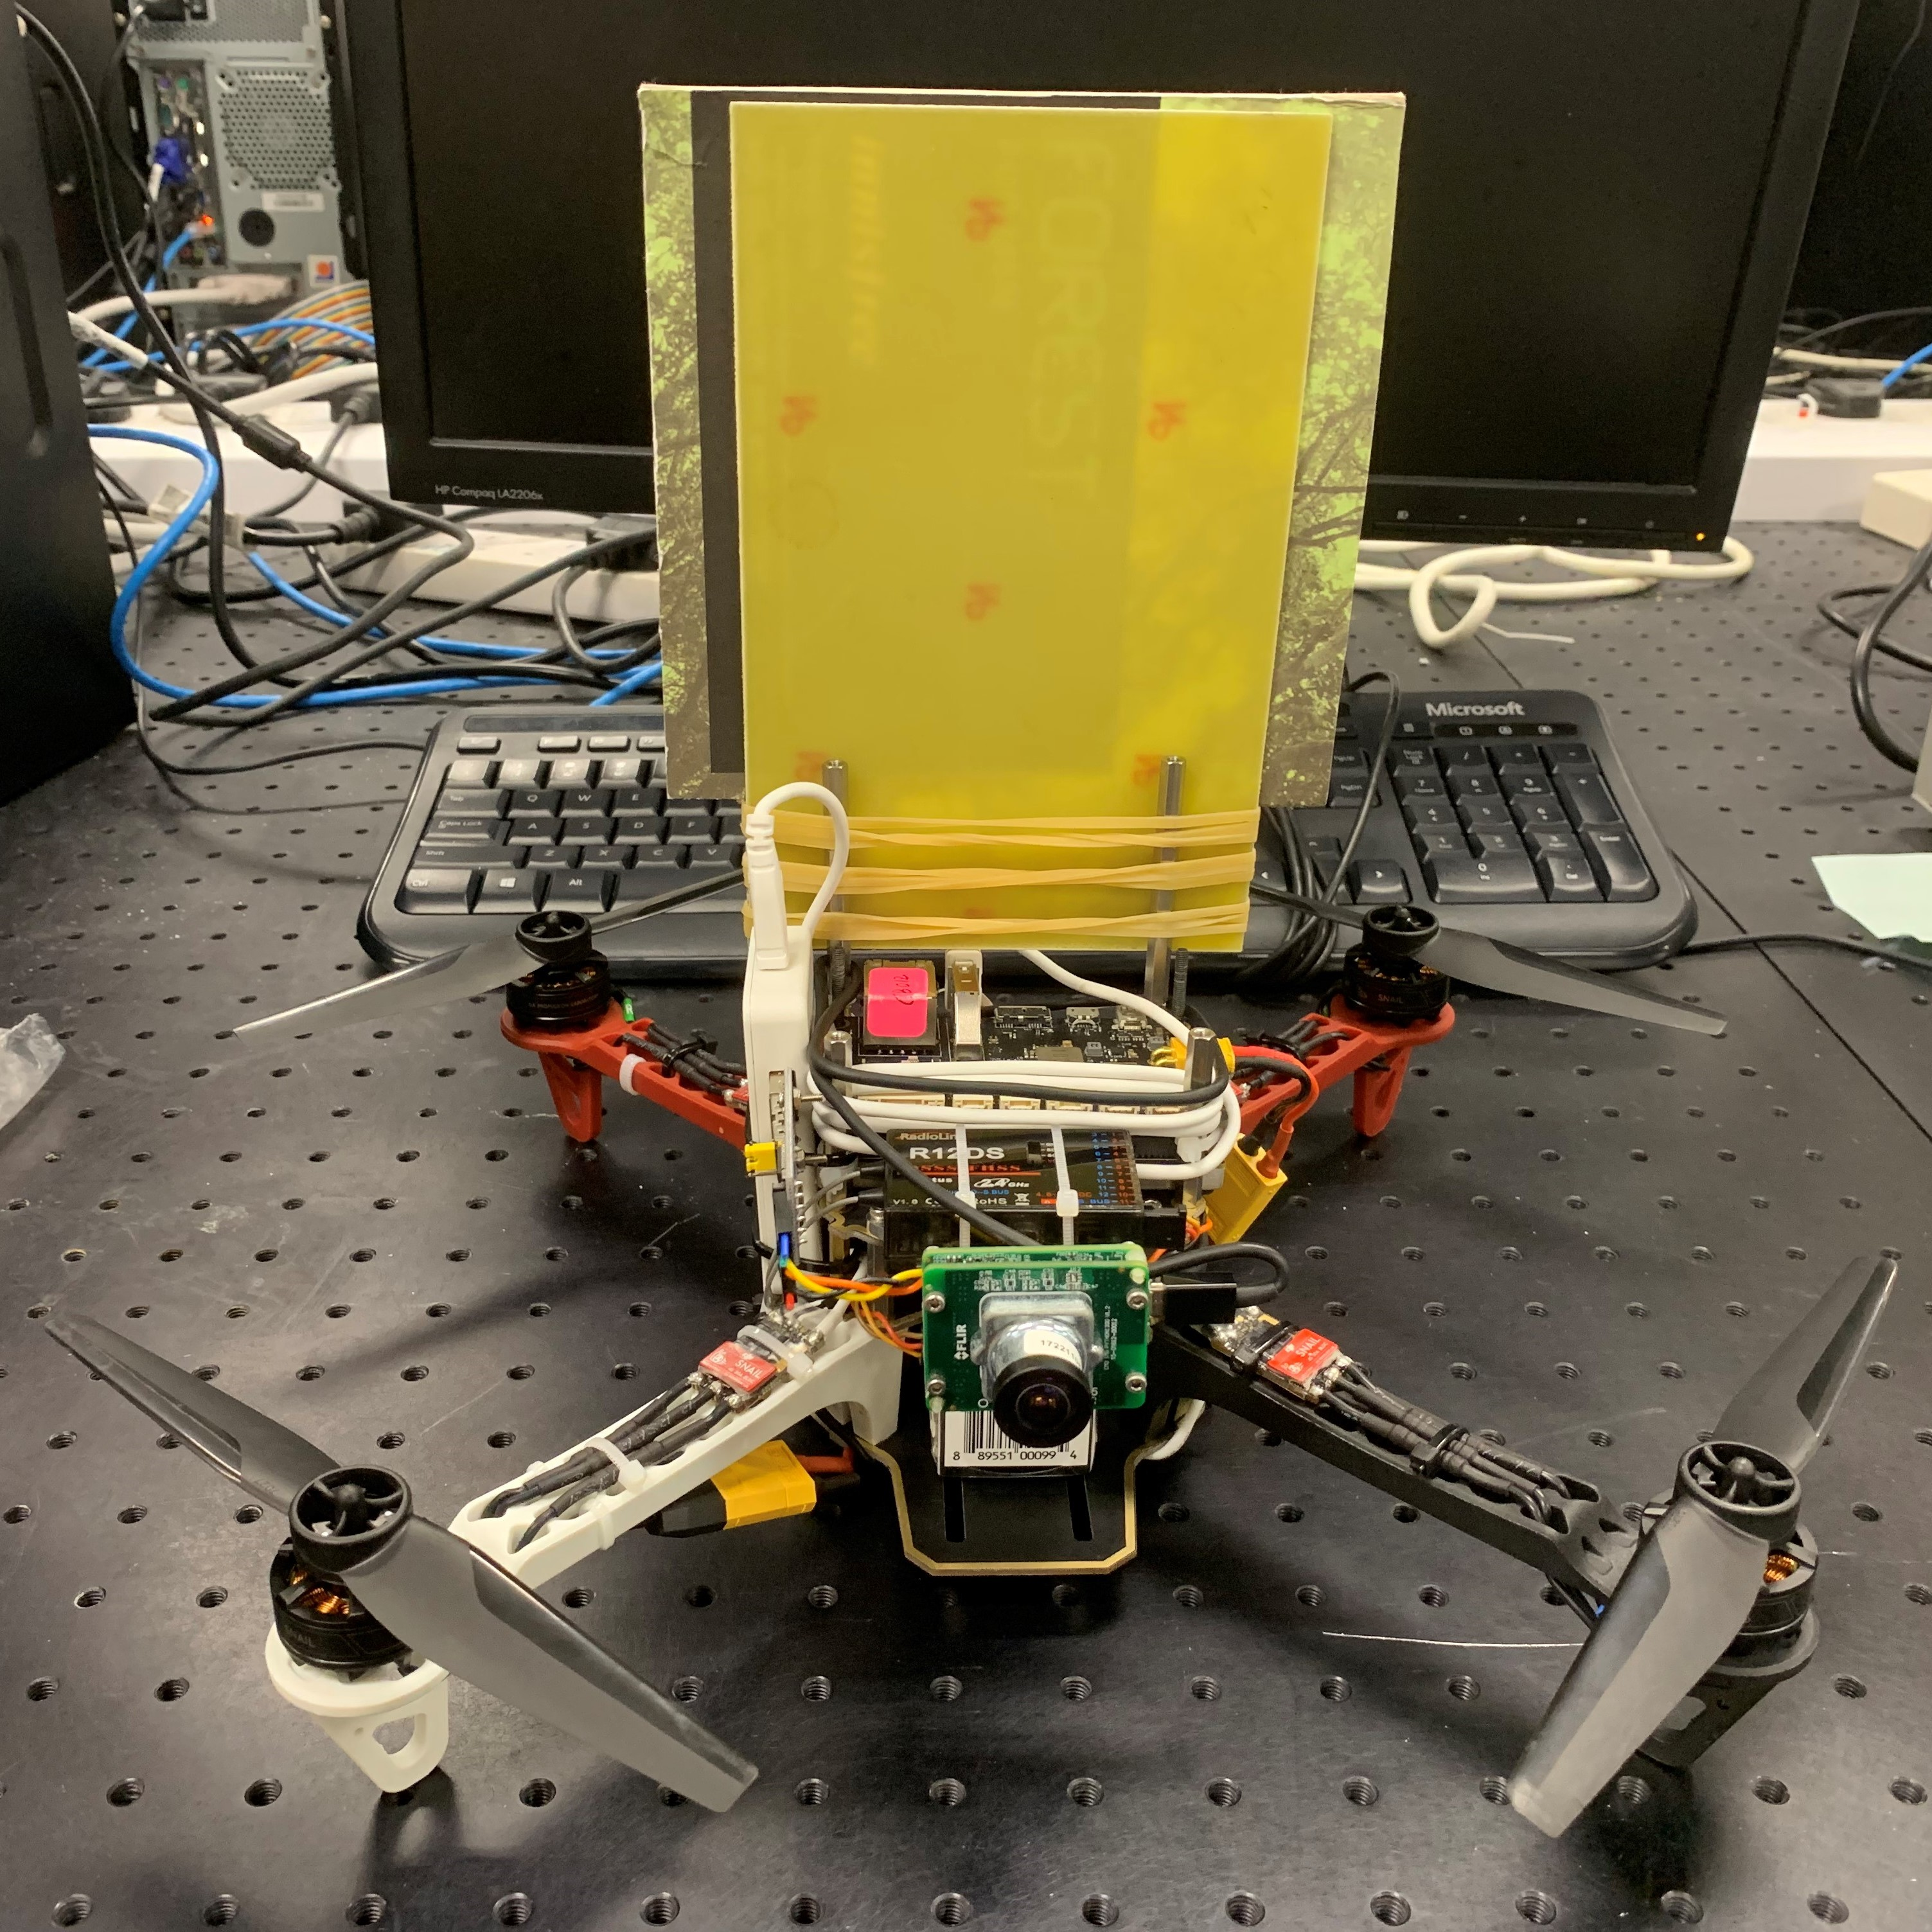
\includegraphics[width=0.49\textwidth]{figure/chapter_4/leader_front.jpg}}
  \caption{Target UAV.}\label{fig:target_uav}
\end{figure}

\begin{table}[htb]
  \centering
 \linespread{1.7}{ {\footnotesize
\vspace{2em}
  \begin{tabular}{ccc}
  \hline
\noalign{\smallskip}
  \textbf{Component} & \textbf{Weight(g)} & \textbf{Power(W)}\\
\noalign{\smallskip}
  \hline
  Intel NUC i5 mini computer & 125 & 15(avg) \\
  Intel Realsense D435i camera & 272 & 2.5(avg) \\
  DJI N3 flight controller & 92 & 3.3(avg)/5(peak) \\
  DJI Lightbridge 2 receiver & 70 &  7.8(avg)\\
\noalign{\smallskip}
  \hline
  \end{tabular}
  }}
  \caption{Weight and power consumption of components on the UAV.}
  \label{tb:weight_power}
\end{table}

\begin{figure}[ht]
  \centering
  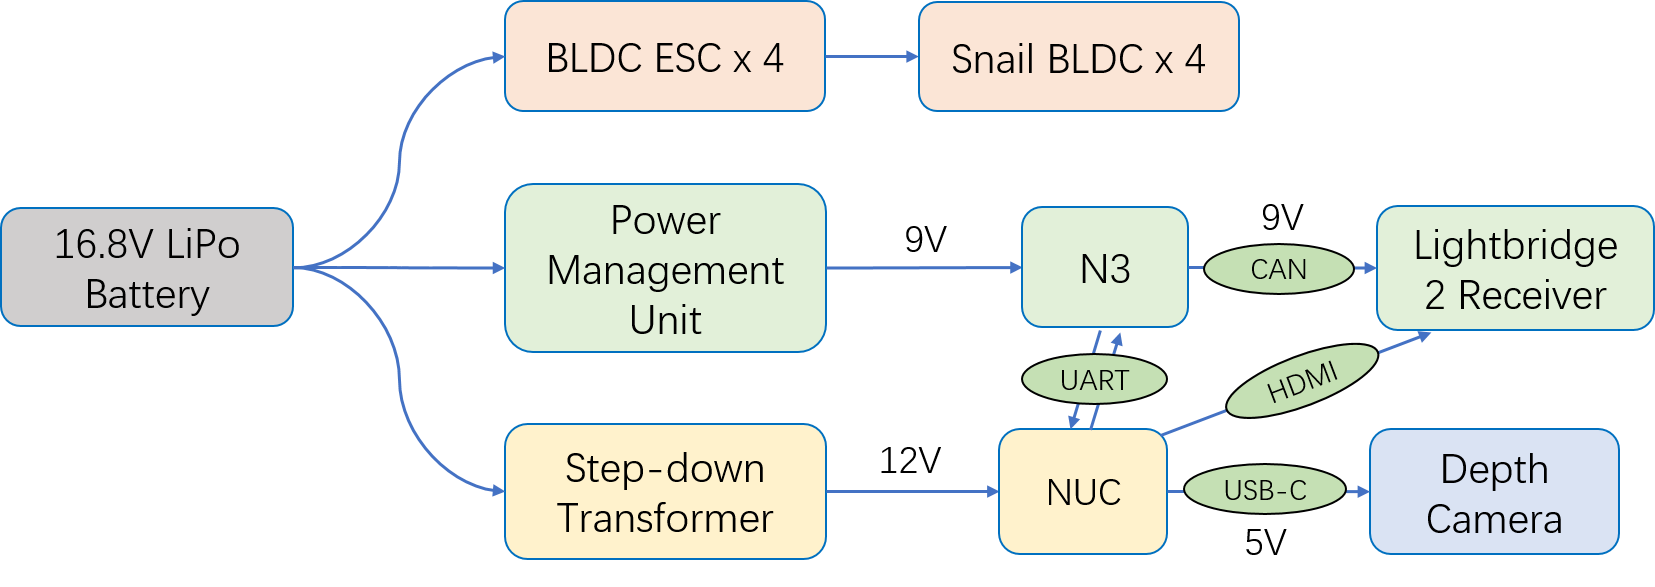
\includegraphics[width=1.0\textwidth]{figure/chapter_4/power_system.png}
  \caption{On-board power systems.}
  \label{fig:power_systems}
\end{figure}

The quadrotor frame consists of the mechanical construction, motors, propellers and the power supply module. Q250 is chosen as the chaser quadrotor frame for its compact size, firm material and the flexibility in maneuvering in cluttered environment. DJI snail BLDC motors and 5 inch 3-blade propellers are mounted for their racing optimized propulsion system and rapid response time. 4S LiPo battery is selected for on-board power supply for its 16.8 V output, 4200 mAh capacity and rechargeable property. The detailed chaser power supply system is illustrated in Figure~\ref{fig:power_systems}. The total weight including the battery is 1.25 kg and the diagonal distance is 25 cm. We use Intel NUC i5 mini computer as our chaser quadrotor main on-board computing resource for both frontend processing and backend optimization. We choose Intel Realsense Depth camera D435i as the forward looking camera for chaser quadrotor's perception and target recognition purposes. It is outfitted with a stereo global shutter camera, with resolution up to 1920x1080 pixels, frame rate up to 90 fps and direct depth map output. More details about on-board components can be found in Table~\ref{tb:weight_power}.

The overall system stability is more emphasized than flexibility on target quadrotor, where F330 frame with diagonal distance of 33 cm, snail BLDC motors and 7 inch propellers are mounted. The demand for computation and perception capability on target quadrotor is lower than the chaser, as its flight path is either controlled by human operator or pre-defined in its on-board computer. In this scenario, NVIDIA Jetson TX2 and Machine Vision Point Grey monocular camera are mounted respectively. DJI N3 flight controller is selected for both chaser and target quadrotor, due to its high quality built-in IMU sensor and compatibility with DJI Lightbridge 2 for live streaming.

\section{Software architecture}\label{software}

\begin{figure}[ht]
  \centering
  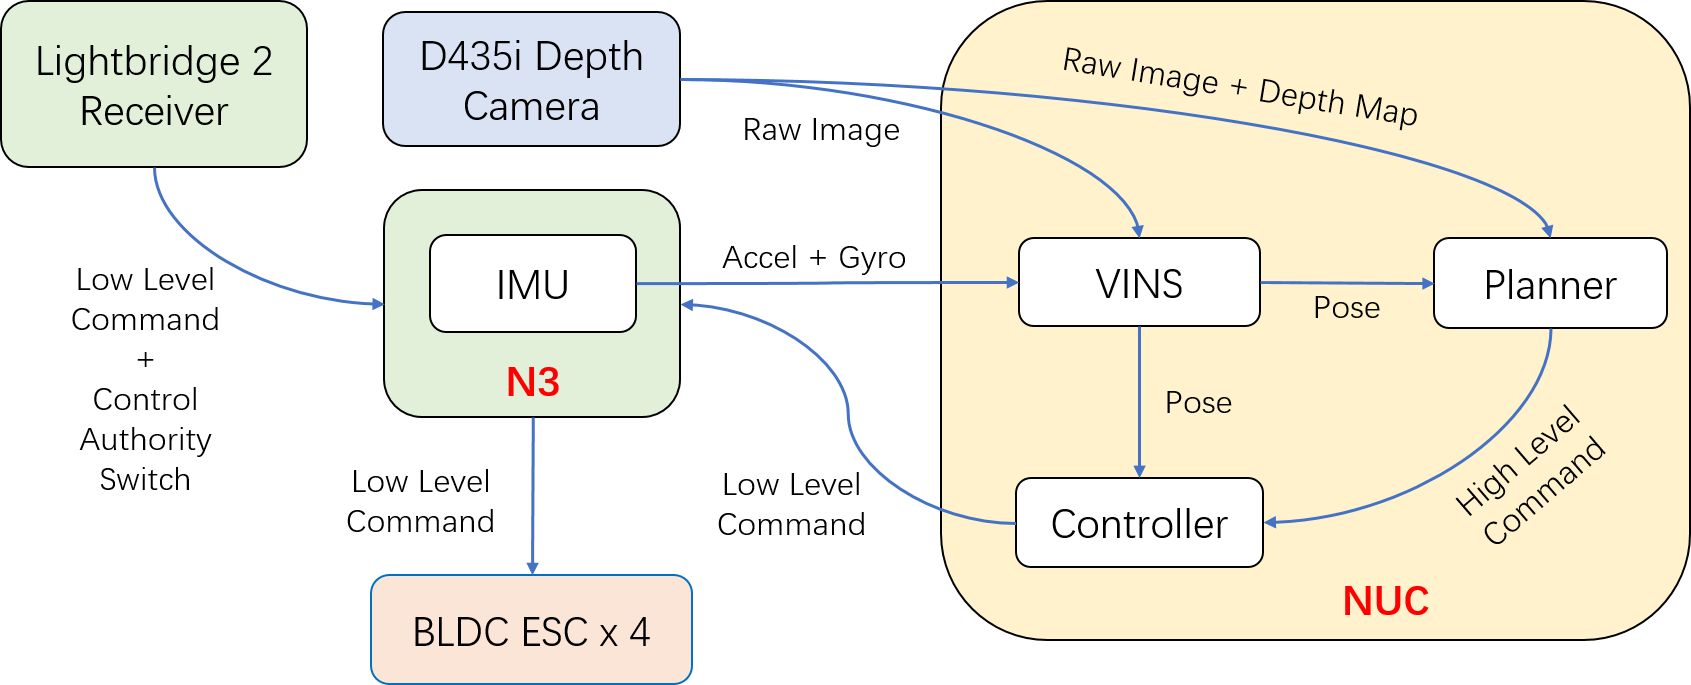
\includegraphics[width=1.0\textwidth]{figure/chapter_4/system_diagram.png}
  \caption{Software architecture}
  \label{fig:software_architecture}
\end{figure}

The software architecture is shown in Figure~\ref{fig:software_architecture}. On chaser's mini i5 computer, 100 Hz IMU measurements and 10 Hz grey scale image data are fused in the visual-inertial state estimator~\cite{VINS} to obtain UAV self position and orientation. Unique aruco code~\cite{Aruco} is attached on target UAV for relative pose estimation and motion prediction. Using predicted target future motion and current chaser pose, a smooth trajectory for chaser UAV is planned and executed with the attitude and thrust control interface in DJI N3 flight controller. Unlike many existing systems that rely on downward facing camera, ultrasonic sensor or LIDAR for sensing, our system only utilize one forward looking camera. We show through both indoor and outdoor experiments that our minimal sensing setup is sufficient for autonomous tracking of an aerial target.

We have also utilized DJI Lightbridge 2 for remote debugging and monitoring. The Lightbridge 2 transforms mini computer's desktop stream to iPad Pro for visualization, including current chaser's pose and live image processing output. This enables us to remotely manipulate the on-board computer while the quadrotor is in the air.

\newpage

\chapter{Experiments and Evaluation}\label{experiment}

\section{Simulation of Flocking Models}

We first show the influence of $\sigma$ and $\beta$ in (\ref{eq:proposed_ui}) to the convergence of the flock by Fig.\ref{fig:sigma_beta}, where the averaged $\psi_{scal}$ (\ref{eq:psi_scal}) of twenty simulation results are illustrated with three cases. The more $\psi_{scal}$ gets close to 1, the more convergent and aligned the flock is. As shown in the figure that the choice of $\sigma$ has little impact on the convergence rate compared with $\beta$. When $\beta\leq\frac{1}{2}$, the convergence of the whole flock is unconditional which is coincident with our assumption in Ch.~\ref{control_law}. Without explicit statement, all the following simulations use $\sigma=1$ and $\beta=0.25$. We then compute the averaged results of $\psi_{scal}$ and relative distance from twenty simulations as illustrated in Fig.\ref{fig:multiple_agent}. We show that the number of total agents in the flock does not influence the characteristics of cohesion, separation and alignment.

\begin{figure}[H]
  \centering
  \subfigure[Average $\psi_{scal}$ of multiple agents with fixed $\sigma, \beta$]{\label{fig:multiple}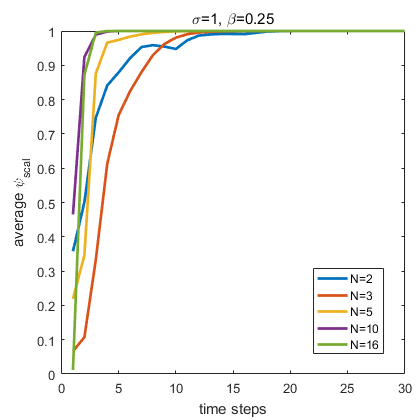
\includegraphics[width=0.49\textwidth]{figure/chapter_5/multiple.png}}
  \subfigure[Average distance of multiple agents with fixed $\sigma, \beta$]{\label{fig:distance}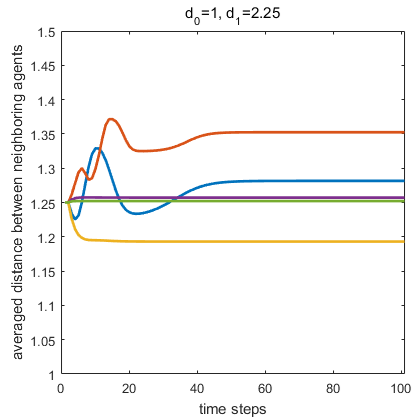
\includegraphics[width=0.49\textwidth]{figure/chapter_5/distance.png}}
  \caption{Average $\psi_{scal}$ and relative distance of multiple agents with fixed $\sigma=1$ and $\beta=0.25$. Their initial velocity are all randomized and nonzero.}\label{fig:multiple_agent}
\end{figure}

\begin{figure}[H]
  \centering
  \subfigure[Case 1: $\sigma<1$ with $\sigma=0.5$]{\label{fig:sigma0_5}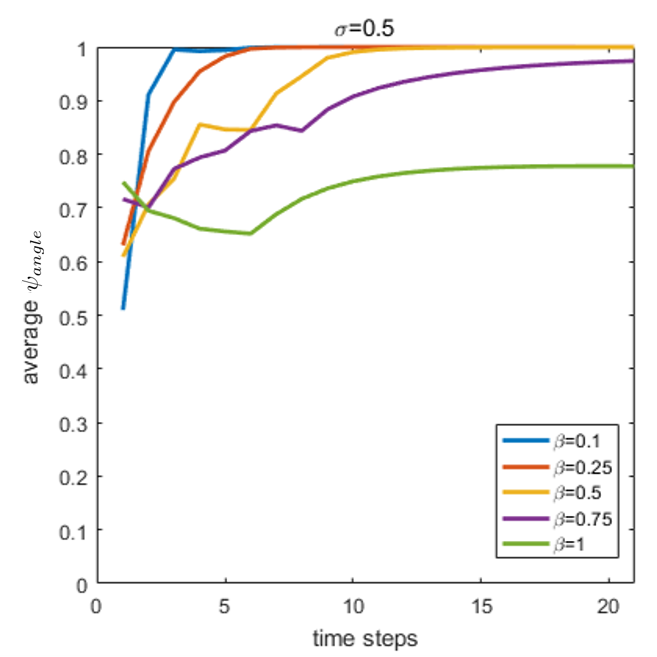
\includegraphics[width=0.49\textwidth]{figure/chapter_5/sigma0_5.png}}
  \subfigure[Case 2: $\sigma=1$]{\label{fig:sigma1}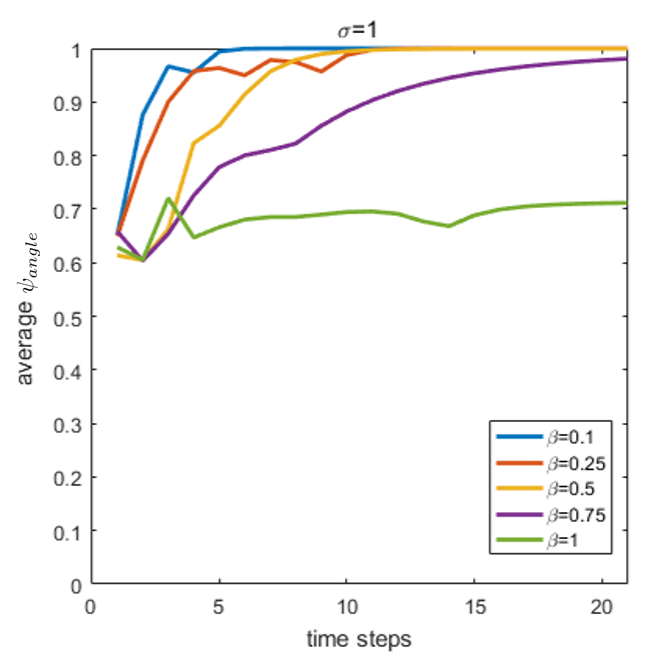
\includegraphics[width=0.49\textwidth]{figure/chapter_5/sigma1.png}}
  \quad
  \subfigure[Case 3: $\sigma>1$ with $\sigma=1.5$]{\label{fig:sigma1_5}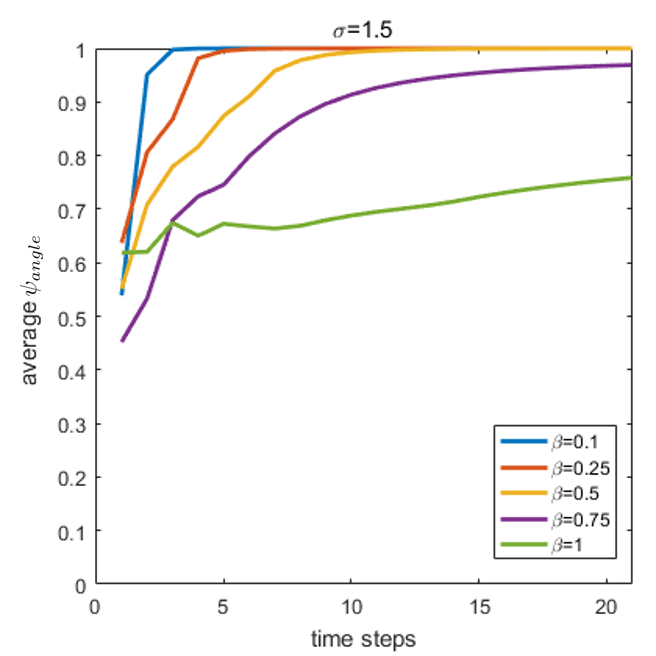
\includegraphics[width=0.49\textwidth]{figure/chapter_5/sigma1_5.png}}
  \caption{Averaged $\psi_{scal}$ of twenty simulations of two agents w.r.t various $\sigma, \beta$. Their initial velocities are all randomized and nonzero.}\label{fig:sigma_beta}
\end{figure}

We compare our proposed flocking model with the ones in~\cite{Vicsek1995,CuckerSmale2007,CuckerDong2010} in Ch.~\ref{flocking} with 2, 3 and 4 agents respectively. The initial position are illustrated in Fig.\ref{fig:simulate_flocking} where the initial velocities are randomized and normalized. The positions of individual agents during the whole simulation are illustrated in Fig.\ref{fig:N_pos} for reference. As illustrated in Fig.\ref{fig:N_scal}, we show that our proposed model converge as fast as those in~\cite{Vicsek1995,CuckerSmale2007,CuckerDong2010}. Especially, we show that the relative distance between neighboring agents in our proposed model is strictly bounded by the interval $(d_0^{\frac{1}{2}}, d_0^{\frac{1}{2}})$. Suppose certain minimum safety distance exists, such as $d_{safe}=0.8$ in Fig.\ref{fig:N3_dis}, our proposed model could successfully avoided collision with neighboring agents. 

\begin{figure}[H]
  \centering
  \subfigure[Two agents in a shape of straight line]{\label{fig:2_agents}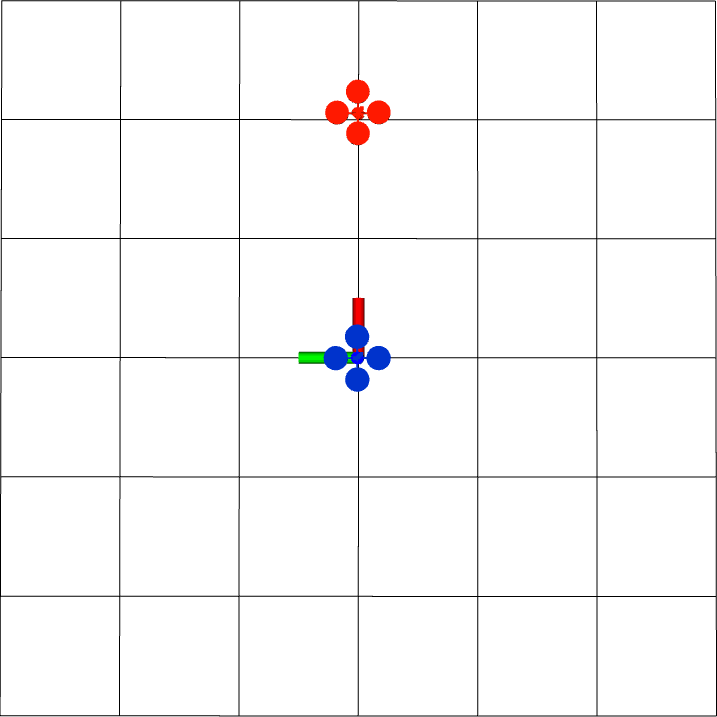
\includegraphics[width=0.32\textwidth]{figure/chapter_5/2_agent.png}}
  \subfigure[Three agents in a shape of equilateral triangle]{\label{fig:2_agents}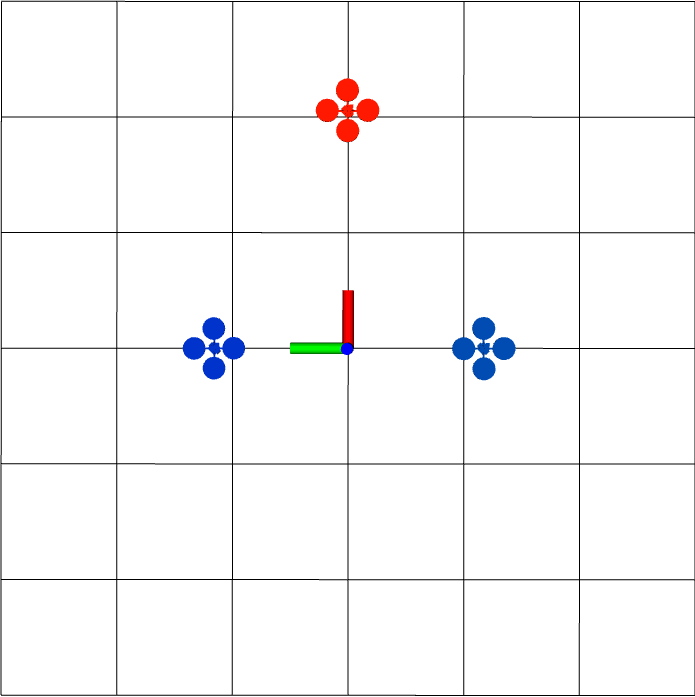
\includegraphics[width=0.32\textwidth]{figure/chapter_5/3_agent.png}}
  \subfigure[Four agents in a shape of diamond]{\label{fig:2_agents}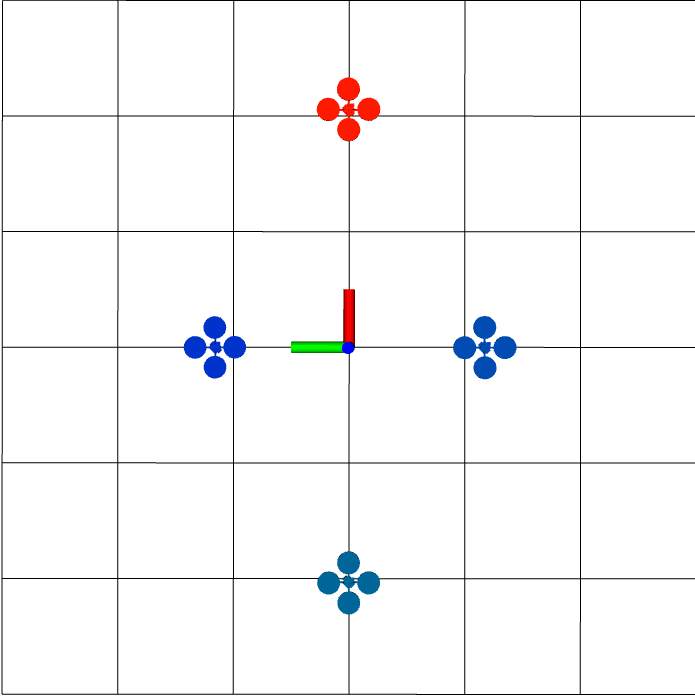
\includegraphics[width=0.32\textwidth]{figure/chapter_5/4_agent.png}}
  \caption{Initial position settings of multi-agent flocking simulations in MATLAB.}\label{fig:simulate_flocking}
\end{figure}

\begin{figure}[H]
  \centering
  \subfigure[$N=2$ agents]{\label{fig:N2_scal}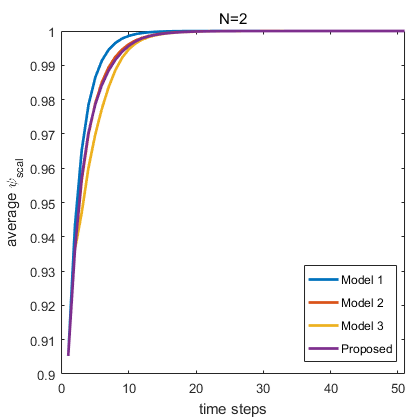
\includegraphics[width=0.49\textwidth]{figure/chapter_5/N2_scal.png}}
  \subfigure[$N=3$ agents]{\label{fig:N3_scal}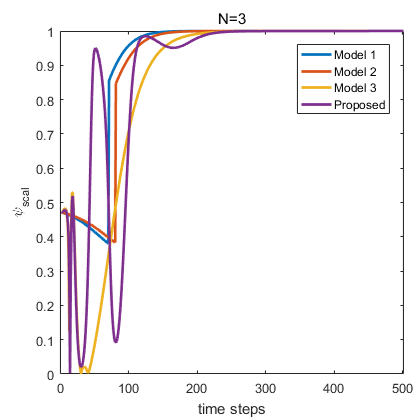
\includegraphics[width=0.49\textwidth]{figure/chapter_5/N3_scal.png}}
  \quad
  \subfigure[$N=4$ agents]{\label{fig:N4_scal}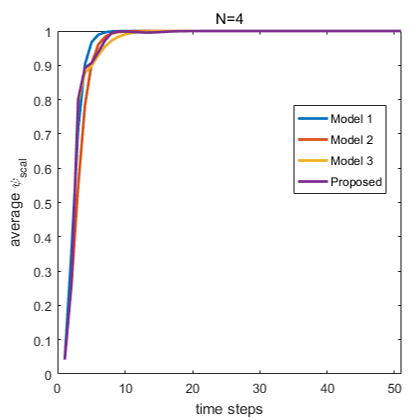
\includegraphics[width=0.49\textwidth]{figure/chapter_5/N4_scal.png}}
  \caption{Convergence descriptor $\psi_{scal}$ of model 1 (\cite{Vicsek1995}), 2 (\cite{CuckerSmale2007}), 3 (\cite{CuckerDong2010}) and our proposed one.}\label{fig:N_scal}
\end{figure}

\begin{figure}[H]
  \centering
  \subfigure[$N=2$ agents.]{\label{fig:N2_dis}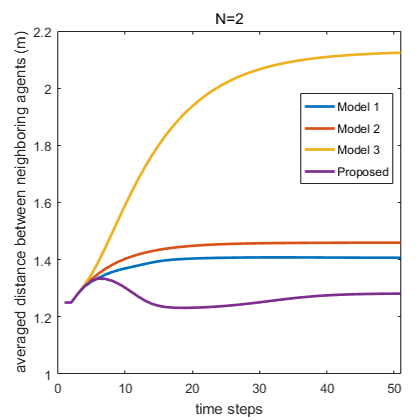
\includegraphics[width=0.49\textwidth]{figure/chapter_5/N2_dis.png}}
  \subfigure[$N=3$ agents.]{\label{fig:N3_dis}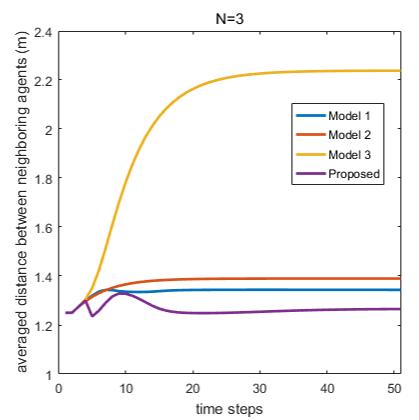
\includegraphics[width=0.49\textwidth]{figure/chapter_5/N3_dis.png}}
  \quad
  \subfigure[$N=4$ agents.]{\label{fig:N4_dis}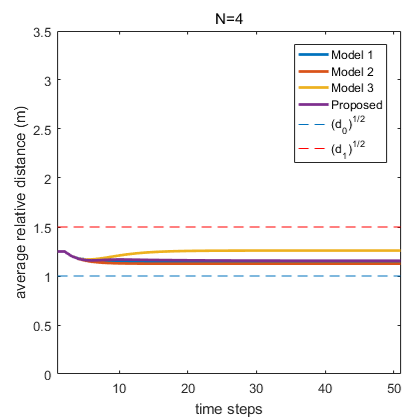
\includegraphics[width=0.49\textwidth]{figure/chapter_5/N4_dis.png}}
  \caption{Average relative distance between neighboring agents. The blue and red dashed line indicate two boundaries $d_0^{\frac{1}{2}}, d_1^{\frac{1}{2}}$ in our proposed model. Model 1, 2 and 3 are from~\cite{Vicsek1995},\cite{CuckerSmale2007} and \cite{CuckerDong2010} respectively.}\label{fig:N_dis}
\end{figure}

\begin{figure}[H]
  \centering
  \subfigure[$N=2$ agents.]{\label{fig:N2_pos}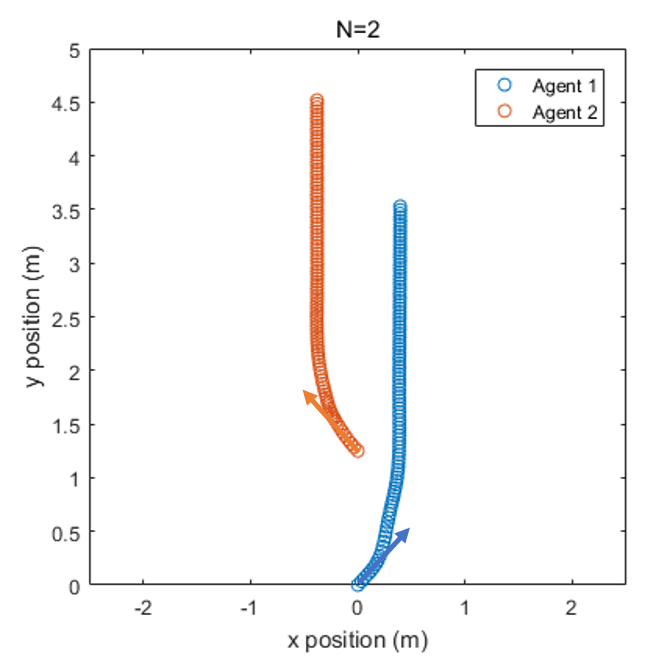
\includegraphics[width=0.49\textwidth]{figure/chapter_5/N2_pos.png}}
  \subfigure[$N=3$ agents.]{\label{fig:N3_pos}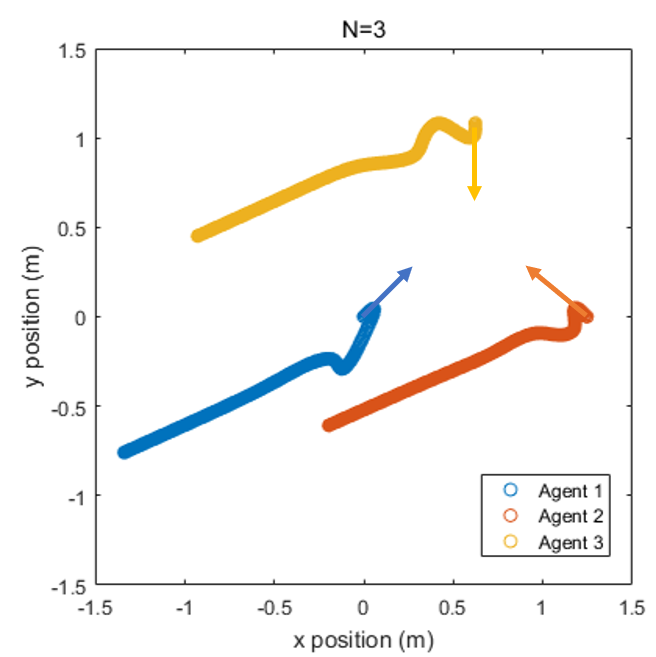
\includegraphics[width=0.49\textwidth]{figure/chapter_5/N3_pos.png}}
  \quad
  \subfigure[$N=4$ agents.]{\label{fig:N4_pos}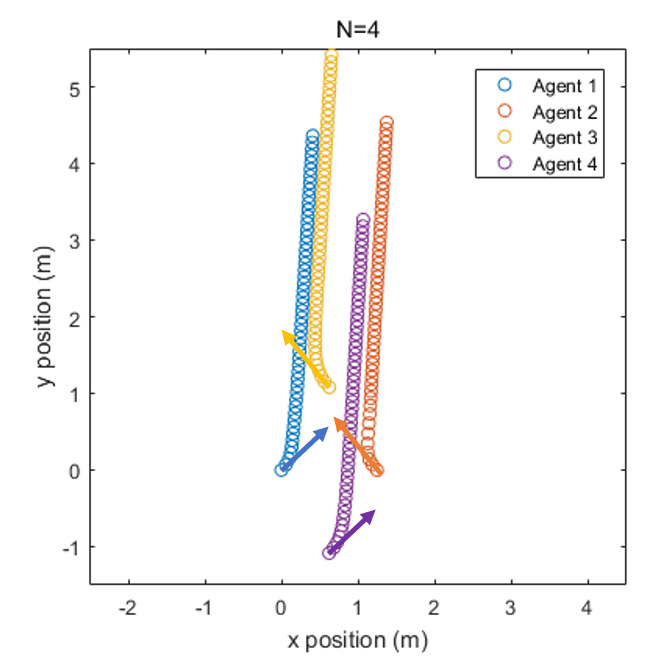
\includegraphics[width=0.49\textwidth]{figure/chapter_5/N4_pos.png}}
  \caption{Motion simulations with normalized initial velocities whose directions are indicated by corresponding arrows.}\label{fig:N_pos}
\end{figure}

\section{Comparison with Tracking Algorithm}\label{tracking}

We have compared the cohesion, separation and alignment performance from our proposed flocking model with those solved by the traditional tracking algorithm. Inspired by~\cite{Chenjing}, we develop a similar method for the chaser UAV to stay $d_s$ away from the target UAV. The entire procedure consists two parts: $\mathit{I}$, target UAV motion estimation and prediction and $\mathit{II}$, chaser UAV trajectory generation. In~\ref{fig:rviz}, the pink arrow (10Hz) indicates the heading of the target UAV and the dark green arrows (400Hz) are the poses of the follower UAV. The light green dots are the 3D positions of the target calculated from captured images, a frame of which is shown in Fig.\ref{fig:capture}. The blue curve and the red one are the predicted path and generated trajectory respectively. As illustrated in Fig.\ref{fig:track_plot}, the developed algorithm has successfully driven the chaser UAV to track the target UAV, however, it is clearly seen in Fig.\ref{fig:position_plot} that the delay is inevitable.

\begin{figure}[htb]
  \centering
  \subfigure[Target motion estimation, prediction and chaser trajectory generation visualized on rviz with data from rosbag.]{\label{fig:rviz}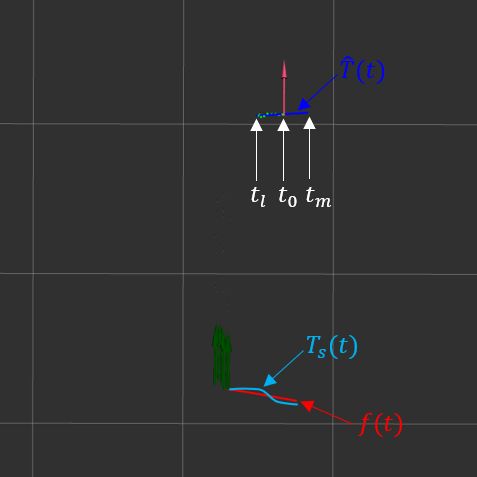
\includegraphics[width=0.49\textwidth]{figure/chapter_5/rviz.png}}
  \subfigure[Image captured from chaser's on-board camera. Green square indicates the recognized aruco code carried on target's UAV.]{\label{fig:capture}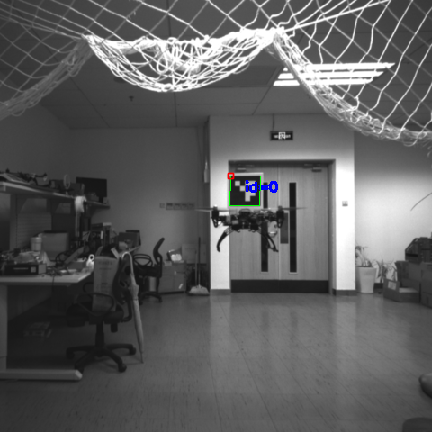
\includegraphics[width=0.49\textwidth]{figure/chapter_5/capture.png}}
  \caption{Screenshots of the tracking algorithm.}\label{fig:rviz_capture}
\end{figure}

\subsection{Target Motion Estimation and Prediction}

We denote the 3D position of the target at time t $\in \mathbb{R}$ as T(t) $\in \mathbb{R}^{3}$ and expand it with Taylor Series. We omit the high order terms $(n>5)$ and approximate it with the $5^{th}$ order polynomial $\hat{T}(t) \in \mathbb{R}^{3}$:

\begin{equation}\label{eq:poly5}
T(t) = \sum^n_{i=0} a_{i}t^i
\approx \sum^5_{i=0} a_{i}t^i
= \begin{bmatrix}1\\t\\t^2\\t^3\\t^4\\t^5\end{bmatrix}^T\begin{bmatrix}a_0\\a_1\\a_2\\a_3\\a_4\\a_5\end{bmatrix}
= T^TA = \hat{T}(t)
\end{equation}

\noindent
Assuming the target's motion is smooth and continuous, we add acceleration regulator $\lambda_{t}$ and minimize the following:

\begin{equation}\label{eq:minT}
\min_{\hat{T}(\cdot)} \sum^{L}_{i=0} ||\hat{T}(t_i)-p_i||^2_2 + \lambda_t\int_{t_l}^{t_m} ||\hat{T}^{(2)}(t)||^2_2dt
\end{equation}

\noindent
where $L$ is the total number of observations captured and $p_i$ is the $i^{th}$ target position in global frame at time $t_i$. Note here that $[t_l, t_0]$ is the time period we actually have target observations and $[t_0, t_m]$ is the period we make predictions for target's motion (\ref{eq:minF}).


\subsection{Trajectory Generation}

During the tracking task, the chaser UAV is expected to keep a fixed distance $d_s\in\mathbb{R}^{3}$ from the target. In this scenario, the chaser UAV is supposed to follow the shifted predicted target trajectory $T_s(t)=\hat{T}(t)+d_s$. Similarly, we denote the planned trajectory for chaser UAV with $f(t)=\sum^5_{i=0} e_{i}t^i=T^TE$ and adjust the tracking stiffness with regulator $\lambda_f$. We then minimize the following:

\begin{equation}\label{eq:minF}
\begin{aligned}
&\min_{f(\cdot)} \int_{t_0}^{t_m} ||f(t)-T_s(t)||^2_{2}dt + \lambda_f\int_{t_0}^{t_m} ||f^{(3)}(t)||^2_{2}dt\\
&s.t.
\end{aligned}
\end{equation}

\begin{equation}
\underbrace{f(t_0)=f_0}_{\text{initial state constraint}}
\end{equation}

\begin{equation}
\underbrace{f(t_m)=0}_{\text{ending state constraint}}
\end{equation}

\begin{equation}
\underbrace{f^{(1)}(t) \in \Omega_{v}(t)}_{\text{velocity constraint}}
\end{equation}

\begin{equation}
\underbrace{f^{(2)}(t) \in \Omega_{a}(t)}_{\text{acceleration constraint}}
\end{equation}

\noindent
where $f_0$ is the state of the chaser UAV at the beginning of the trajectory and $\Omega_v$ and $\Omega_a$ are the velocity and acceleration constraints respectively.

We can rewrite (\ref{eq:minF}) as:

\begin{equation}\label{eq:reminF1}
\min_{l\in\{x,y,z\}}\int_{0}^{t_m-t_0} (A^TT_sT_s^TA-2E^TT^TT_s^TA+E^TT^TTE)dt + \lambda_f\int_{0}^{t_m-t_0} (E^TT_fT_f^TE)dt\\
\end{equation}

\noindent
and transform (\ref{eq:reminF1}) into a standard QP problem:

\begin{equation}\label{eq:reminF2}
\min_{l\in\{x,y,z\}}E^T[\int_{0}^{t_m-t_0}(T^TT+T_fT_f^T)dt]E-2E^T[\int_{0}^{t_m-t_0}T_f^TT_s^T]A
\end{equation}

\noindent
where $T_s = \begin{bmatrix}1\\1+dT\\(1+dT)^2\\(1+dT)^3\\(1+dT)^4\\(1+dT)^5\end{bmatrix}$ and $T_f=\begin{bmatrix}0\\0\\0\\6\\24t\\60t^2\end{bmatrix}$ with $dT=t_0-t_l$. We use $l\in\{x,y,z\}$ to abstract the dimension.

\subsection{Tracking Performance}

\begin{figure}[H]
  \centering
  \subfigure[Position profiles of target and chaser UAVs. The blue and red lines are the x and y positions of the target UAV and the yellow and the purple lines are the x and y positions of the chaser UAV.]{\label{fig:position_plot}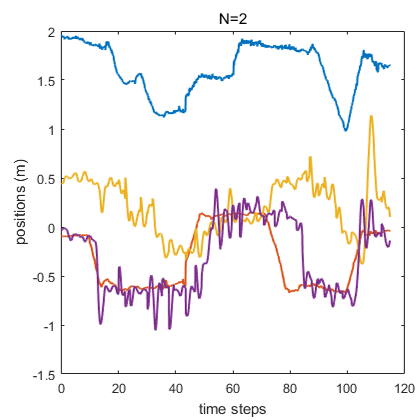
\includegraphics[width=0.49\textwidth]{figure/chapter_5/position_plot.png}}
  \subfigure[Relative distance between target and chaser UAVs. The desired shifted distance $d_s=1.5$ while the averaged relative distance $\bar{d}=1.39$.]{\label{fig:distance_plot}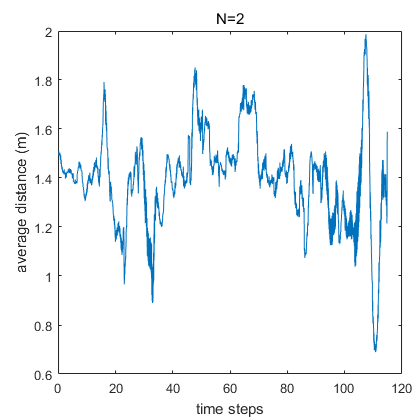
\includegraphics[width=0.49\textwidth]{figure/chapter_5/distance_plot.png}}
  \quad
  \subfigure[$\psi_{scal}$ of the tracking system.]{\label{fig:scal_plot}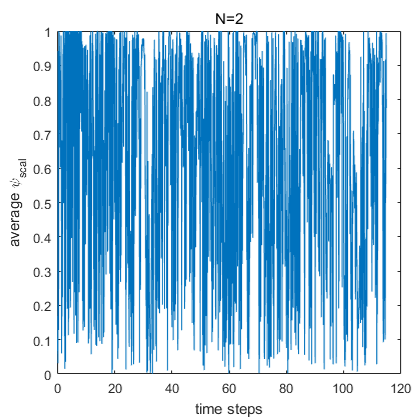
\includegraphics[width=0.49\textwidth]{figure/chapter_5/scal_plot.png}}
  \caption{\textcolor{red}{TODO: Modify $\psi_{scal}$ plot.}}\label{fig:track_plot}
\end{figure}

\section{Realization of Proposed Model}

\begin{figure}[H]
  \centering
  \subfigure[Position profiles of leader and follower UAVs. The yellow and purple lines are the x and y positions of the leader UAV and the blue and the red lines are the x and y positions of the follower UAV.]{\label{fig:x_indoor_position}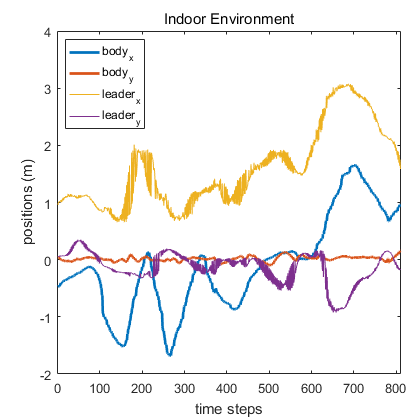
\includegraphics[width=0.49\textwidth]{figure/chapter_5/x_indoor_position.png}}
  \subfigure[Relative distance between leader and follower UAVs.]{\label{fig:x_indoor_distance}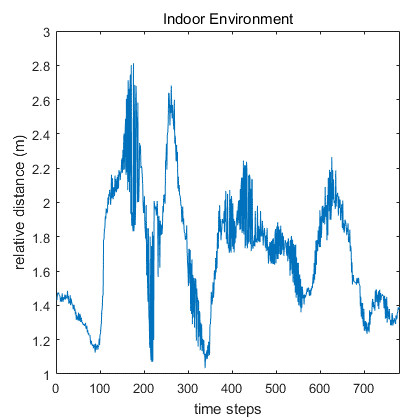
\includegraphics[width=0.49\textwidth]{figure/chapter_5/x_indoor_distance.png}}
  \quad
  \subfigure[$\psi_{scal}$]{\label{fig:x_indoor_scal}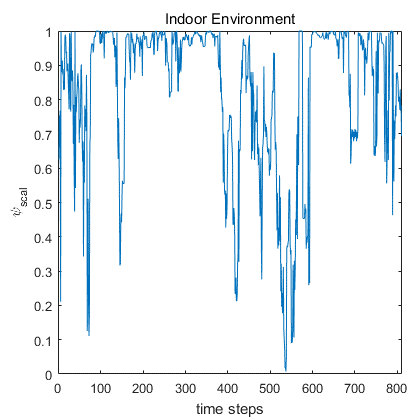
\includegraphics[width=0.49\textwidth]{figure/chapter_5/x_indoor_scal.png}}
  \caption{\textcolor{red}{TODO.}}\label{fig:x_indoor}
\end{figure}

\newpage

\chapter{Conclusion}\label{conclusion}

In this thesis, a flocking system consisting two quadrotors based on mathematical control model is presented and the detailed hardware and software platforms are introduced. The leader UAV is manually controlled, the follower UAV could be switched to autonomous mode and stay flocking with the leader. The monocular camera is used as the only on-board sensor for both follower UAV state estimation and leader UAV pose recognition. When the flocking begins, the follower UAV first percepts the surrounding environment to estimate self-state, then recognize leader UAV's pose and calculate desired acceleration using our proposed model and third execute the desired input until next image is captured and processed.

Simulations, real world experiments and the comparison of the results from tracking algorithm with our proposed method have been conducted and analysed. We have shown that our flocking system has met the three flocking criteria without relying on any external perception system or central control panel, achieved relatively faster convergence rate and kept bounded relative distance with neighboring agents to avoid collision, given fine weather conditions.

Our future work will focus on the flocking of more than two quadrotors in GPS-denied environment, including introducing multiple fisheye cameras or an omnidirectional camera for perception and the study of ultra wide band (UWB) method for relative distance measurement and internal communication.


%%%%%%%%%%%%%%%%%%%%%%%%%%%%%%%%%%%%%%%%%%%%%%%%%%%%%%%%%%%%%%%%%%%%%%%%%
%                                                                       %
%      9) BIBLIOGRAPHY                                                  %
%                                                                       %
% This example uses bibtex to generate the required Bibliography. Refer %
% to the % the file ustthesis_test.bib for the entries of the           %
% Bibliography. Note that only the cited entries are printed.           %
%                                                                       %
% If BibTeX is not used to typeset the bibliography, replace the        %
% following line with the \begin{thebibliography} and \end{bibliography}%
% commands (the "thebibliography" environment) to process the           %
% Bibliography.                                                         %
%                                                                       %
%%%%%%%%%%%%%%%%%%%%%%%%%%%%%%%%%%%%%%%%%%%%%%%%%%%%%%%%%%%%%%%%%%%%%%%%%

%%%%%%%%%%%%%%%%%%%%%%%%%%%%%%%%%%%%%%%%%%%%%%%%%%%%%%%%%%%%%%%%%%%%%%%%%
%                                                                       %
% The recommended bibliography style is the IEEE bibliography style.    %
% "ustbib" defines the IEEE bibliography standard with the added        %
% ability of sorting the items by name of author.                       %
%                                                                       %
% If you are not using BibTeX to process your Bibliography, comment out %
% the following line.                                                   %
%                                                                       %
%%%%%%%%%%%%%%%%%%%%%%%%%%%%%%%%%%%%%%%%%%%%%%%%%%%%%%%%%%%%%%%%%%%%%%%%%

\bibliographystyle{plain}


\bibliography{ref}
% Please run "bibtex ustthesis_test" before the bibliography can be
% included.

%%%%%%%%%%%%%%%%%%%%%%%%%%%%%%%%%%%%%%%%%%%%%%%%%%%%%%%%%%%%%%%%%%%%%%%%%
%                                                                       %
%     10) APPENDIX (If Any)                                              %
%                                                                       %
% \appendix command marks the beginning of the APPENDIX part of the     %
% Thesis. The usual \chapter command is used for the different chapters %
% of the Appendix.                                                      %
%                                                                       %
%%%%%%%%%%%%%%%%%%%%%%%%%%%%%%%%%%%%%%%%%%%%%%%%%%%%%%%%%%%%%%%%%%%%%%%%%


%%%%%%%%%%%%%%%%%%%%%%%%%%%%%%%%%%%%%%%%%%%%%%%%%%%%%%%%%%%%%%%%%%%%%%%%%
%                                                                       %
%     11) BIOGRAPHY (Optional)                                          %
%                                                                       %
% \biography and \endbiography are used to define the optional          %
% Biography of the author of the Thesis.                                %
%                                                                       %
%%%%%%%%%%%%%%%%%%%%%%%%%%%%%%%%%%%%%%%%%%%%%%%%%%%%%%%%%%%%%%%%%%%%%%%%%

% \biography
% The biography of the student is ALSO optional.
% \endbiography

\end{document}
\grid
